
\documentclass[aspectratio=169, 10pt]{beamer}
\usetheme{metropolis} % or \usetheme{moloch}

% Optional: Fira Sans font (standard for Metropolis)
\usepackage[sfdefault]{FiraSans}
\usepackage{FiraMono}

\metroset{
  progressbar=frametitle,
  block=fill,
  numbering=fraction
}

% Metropolis omits frame subtitles; add them inside its existing title bar.
\setbeamerfont{framesubtitle}{size=\scriptsize,series=\mdseries}
\makeatletter
\patchcmd{\beamer@@tmpl@frametitle}
{\insertframetitle}
{\insertframetitle%
  \ifx\insertframesubtitle\@empty\else
  \par\usebeamerfont{framesubtitle}\insertframesubtitle
\fi}
{}
{\PackageError{Thomson}{Could not enable frame subtitles}{Check the Metropolis frametitle template.}}
\makeatother

% Use scriptsize throughout, including headings and nested lists.
\setbeamerfont{normal text}{size=\scriptsize}
\AtBeginDocument{\usebeamerfont{normal text}}
\AtBeginEnvironment{frame}{\scriptsize}
\newcommand{\scriptsizebeamerfont}[1]{\setbeamerfont{#1}{size=\scriptsize}}
\forcsvlist{\scriptsizebeamerfont}{title,subtitle,author,institute,date,frametitle,framesubtitle,section title,subsection title,section in toc,subsection in toc,subsubsection in toc,block title,block body,block title alerted,block body alerted,block title example,block body example,itemize/enumerate body,itemize/enumerate subbody,itemize/enumerate subsubbody,caption,caption name,footnote,footline,page number in head/foot,bibliography entry author,bibliography entry title,bibliography entry location,bibliography entry note}

% Custom refined palette (Deep Slate & Muted Amber)
\definecolor{DarkSlate}{HTML}{1F2D3D}
\definecolor{AmberAlert}{HTML}{D97706}
\setbeamercolor{palette primary}{bg=DarkSlate, fg=white}
\setbeamercolor{alerted text}{fg=AmberAlert}

% Reusable visual treatment for numerical validation results.
\definecolor{ValidationTeal}{HTML}{167D8D}
% Restrained accents for theory; stronger teal remains reserved for tests.
\setbeamercolor{structure}{fg=ValidationTeal}
\setbeamercolor{block title}{fg=DarkSlate,bg=ValidationTeal!12!white}
\setbeamercolor{block body}{fg=DarkSlate,bg=ValidationTeal!4!white}
\setbeamercolor{equation panel}{fg=DarkSlate,bg=ValidationTeal!5!white}
\newcommand{\theorylabel}[1]{{\color{ValidationTeal}\textbf{#1}}}
\newenvironment{equationpanel}{%
  \par
  \begin{beamercolorbox}[wd=\linewidth,sep=0pt]{equation panel}%
  }{%
  \end{beamercolorbox}%
}
\newenvironment{validationtest}[2]{%
  \begingroup
  \setbeamercolor{block title example}{fg=white,bg=ValidationTeal}
  \setbeamercolor{block body example}{fg=DarkSlate,bg=ValidationTeal!8!white}
  \begin{exampleblock}{Validation test #1 --- #2}%
  }{%
  \end{exampleblock}
  \endgroup
}

\title{Non linear Thomson Scattering}
\author{Gabriel Majeri, Virgil Baran, Madalina Boca}

\begin{document}
\begin{frame}{}
  \maketitle

\end{frame}

\begin{frame}{}
  \tableofcontents
\end{frame}
\section{The Laguerre Gaussian modes of the electromagnetic field}
\begin{frame}{The Laguerre Gaussian modes of the electromagnetic field}
  \framesubtitle{The scalar solution}
  \begin{align*}
    u_{pm}({\bf r}) = N_{pm}\frac{w_0}{w(z)}\left(\frac{\sqrt{2}}{w(z)}\right)^me^{-i(2p + m +1)\psi_G(z)}e^{-\frac{k}2\frac{x^2+y^2}{z_R+i z}}\, _1F_1(-p, m+1, \frac{2(x^2+y^2)}{w(z)^2}) (x+i\epsilon y)^m,
  \end{align*}
  \begin{itemize}
    \item  $E_0 = \omega \xi \frac{mc}{|e|}$
    \item $w_0$ = the beam waist
    \item $z_R = \frac{kw_0^2}{2}$ = the Rayleigh length
    \item $w(z) = w_0\sqrt{1+\frac{z^2}{z_R^2}}$
    \item $\psi_G(z) = \arctan\frac{z}{z_R}$
    \item $\epsilon=\pm1$ helicity sign
    \item $\zeta_x$, $\zeta_y$ polarization parameters $|\zeta_x|^2 + |\zeta_y|^2=1$
    \item $N_{pm} = \frac{\sqrt{2}}{m!}\sqrt{\frac{(p+m)!}{p!}}$ normalization constant

  \end{itemize}

\end{frame}
\begin{frame}{The Laguerre Gaussian modes of the electromagnetic field}
  \framesubtitle{The electromagnetic field}
  \begin{align*}
    & E_x({\bf r},t) = E_0\Re\left\{\zeta_x u_{pm}({\bf r})f(\phi)\right\},\quad f(\phi)=e^{-i\phi-\frac{(\phi -  \tau_0)^2 }{\tau^2}},\quad \phi = \omega t-kz                  \\
    & E_y({\bf r},t) = E_0\Re\left\{\zeta_y u_{pm}({\bf r})f(\phi)\right\}                                                                                                       \\
    & E_z({\bf r},t) = E_0\Re\left\{-\frac1{ik}\left[\zeta_x\frac{\partial u_{pm}({\bf r})}{\partial x}+\zeta_y\frac{\partial u_{pm}({\bf r})}{\partial y}\right]f(\phi)\right\}\\
    & B_x({\bf r},t) = \frac{E_0}c\Re\left\{-\zeta_y u_{pm}({\bf r})f(\phi)\right\},\quad f(\phi)=e^{-i\phi-\frac{(\phi -  \tau)^2 }{\tau^2}},\quad \phi = \omega t-kz                    \\
    & B_y({\bf r},t) = \frac{E_0}c\Re\left\{\zeta_x u_{pm}({\bf r})f(\phi)\right\}                                                                                                        \\
    & B_z({\bf r},t) = \frac{E_0}c\Re\left\{-\frac1{ik}\left[-\zeta_y\frac{\partial u_{pm}({\bf r})}{\partial x}+\zeta_x\frac{\partial u_{pm}({\bf r})}{\partial y}\right]f(\phi)\right\}
  \end{align*}
\end{frame}
\begin{frame}{The Laguerre Gaussian modes of the electromagnetic field}

  Plots of the incident field for $p=m=2$, circular polarization: Gaussian wings with $\sigma=5$, flat top duration $=50$ cycles.

  \vspace{0.5cm}

  \centering
  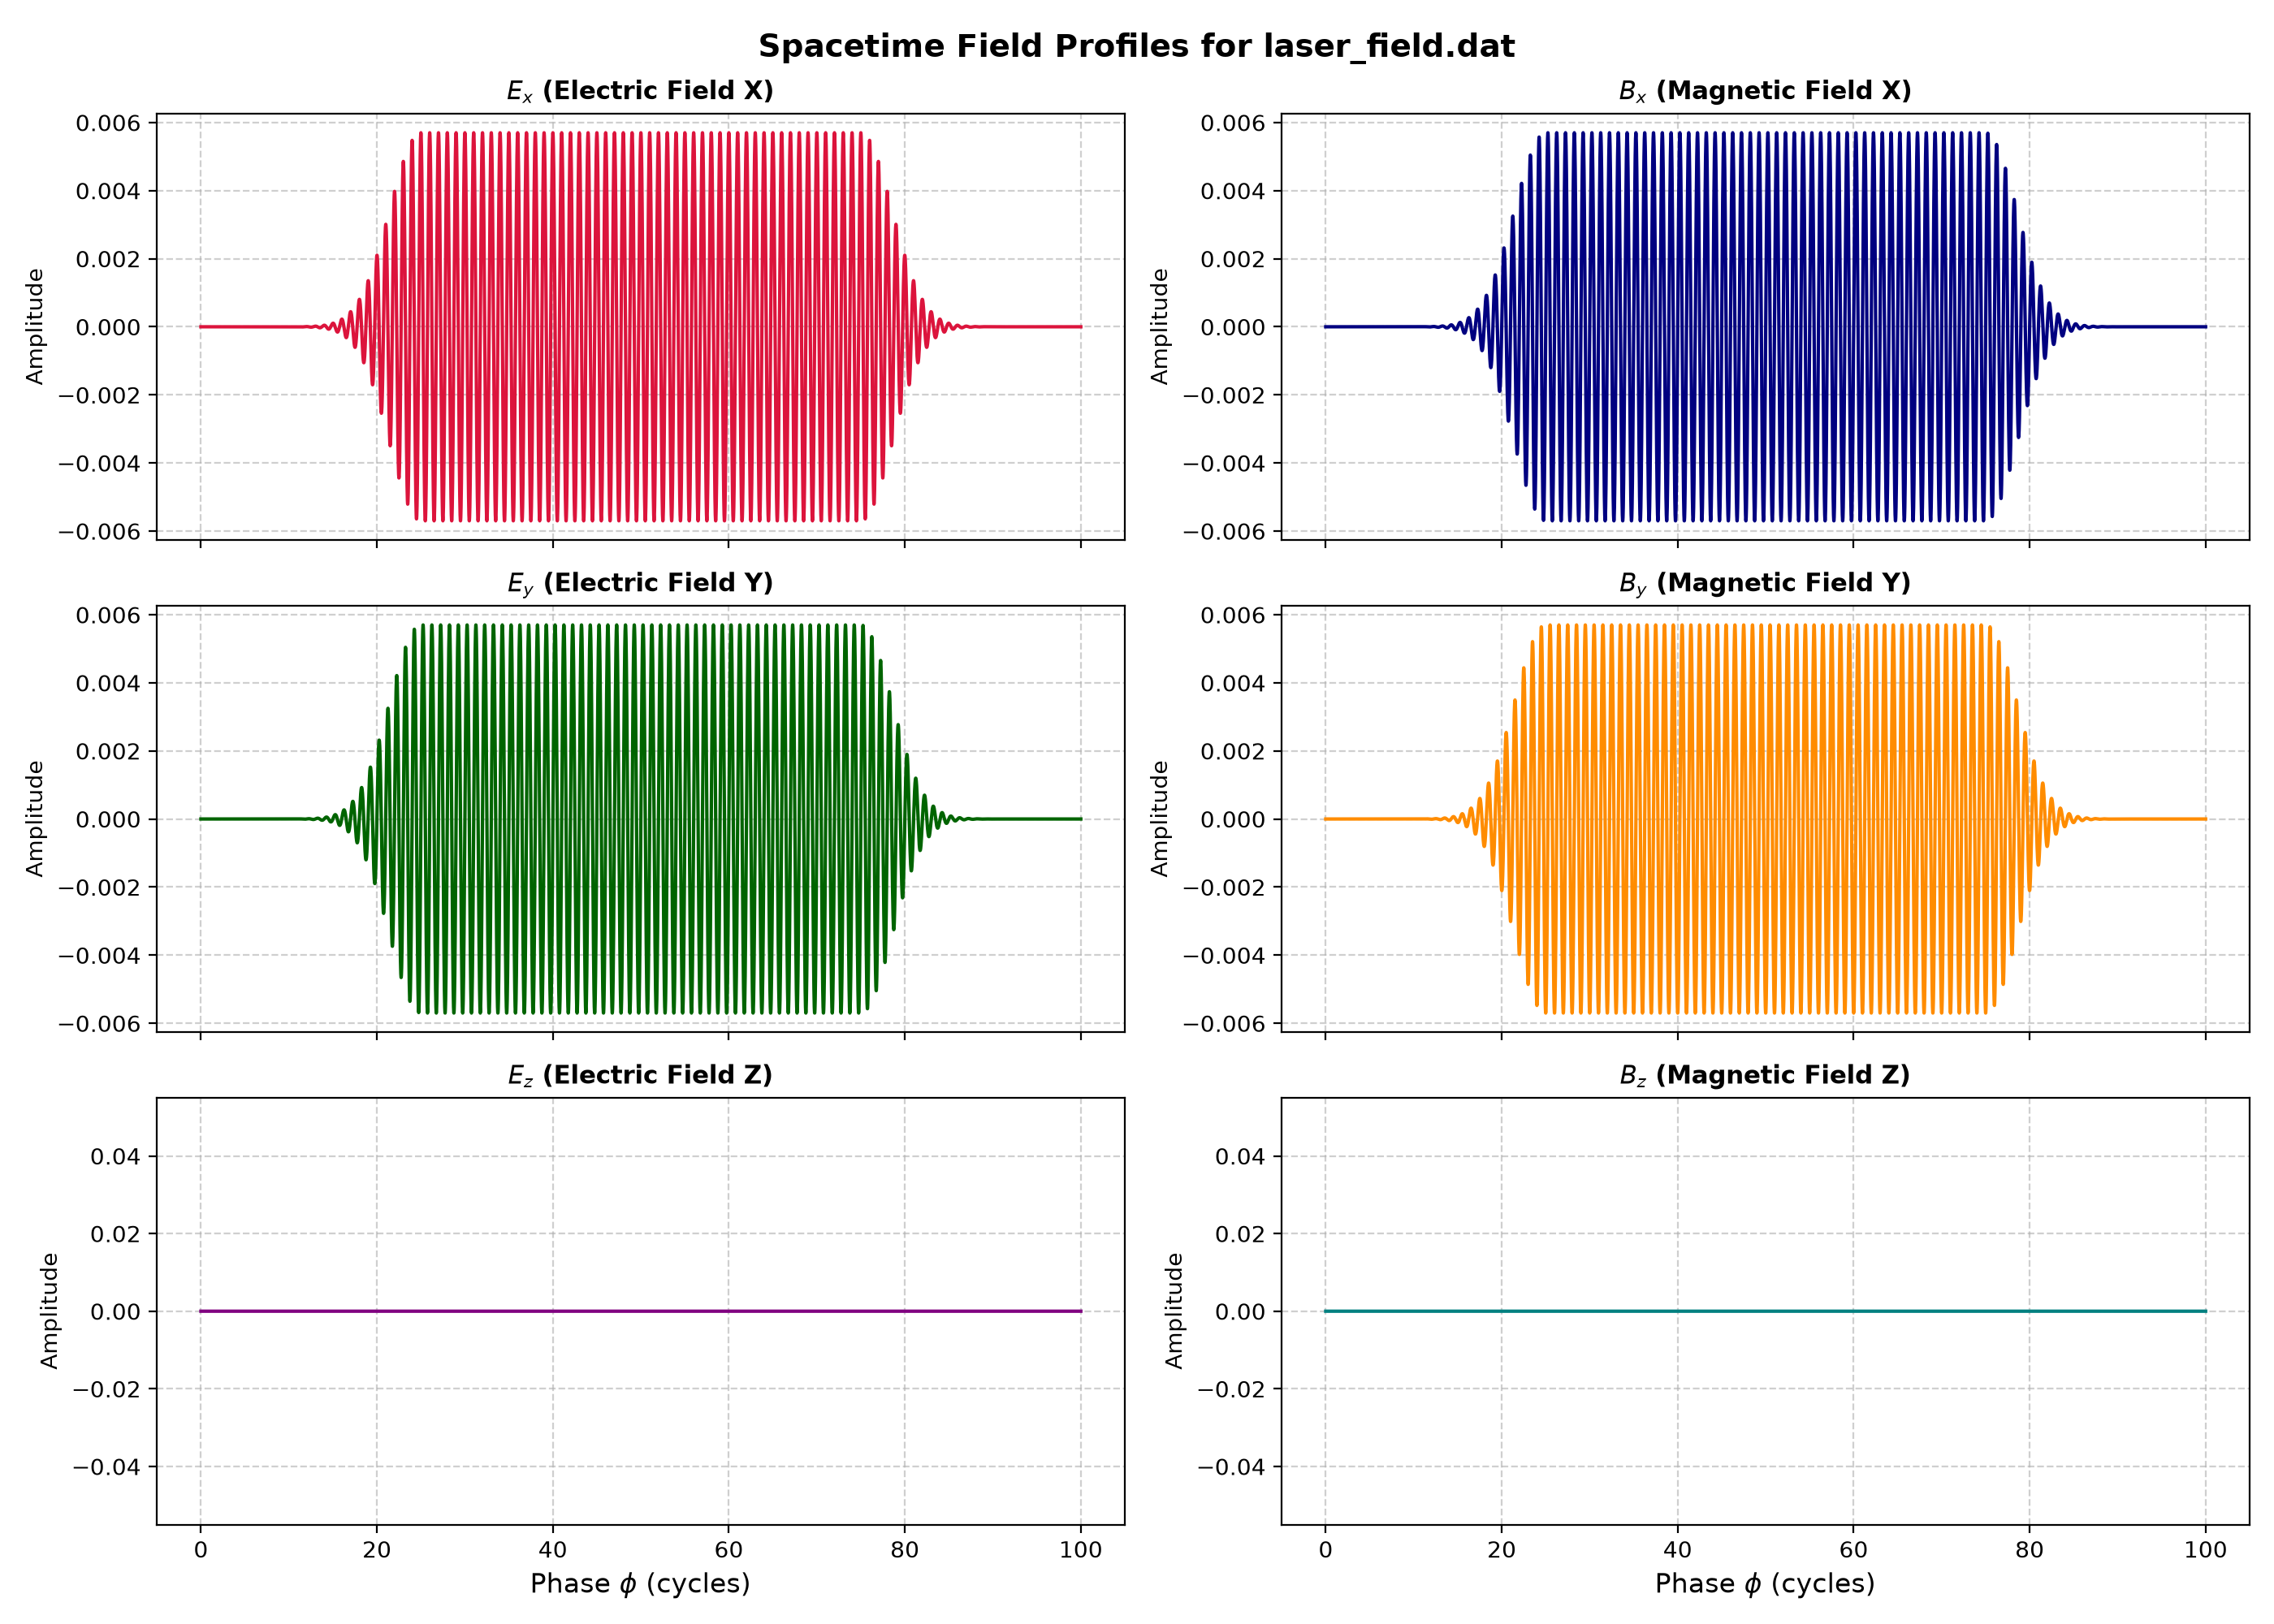
\includegraphics[height=0.62\textheight]{figs/laser_field_profile.png}\hfill
  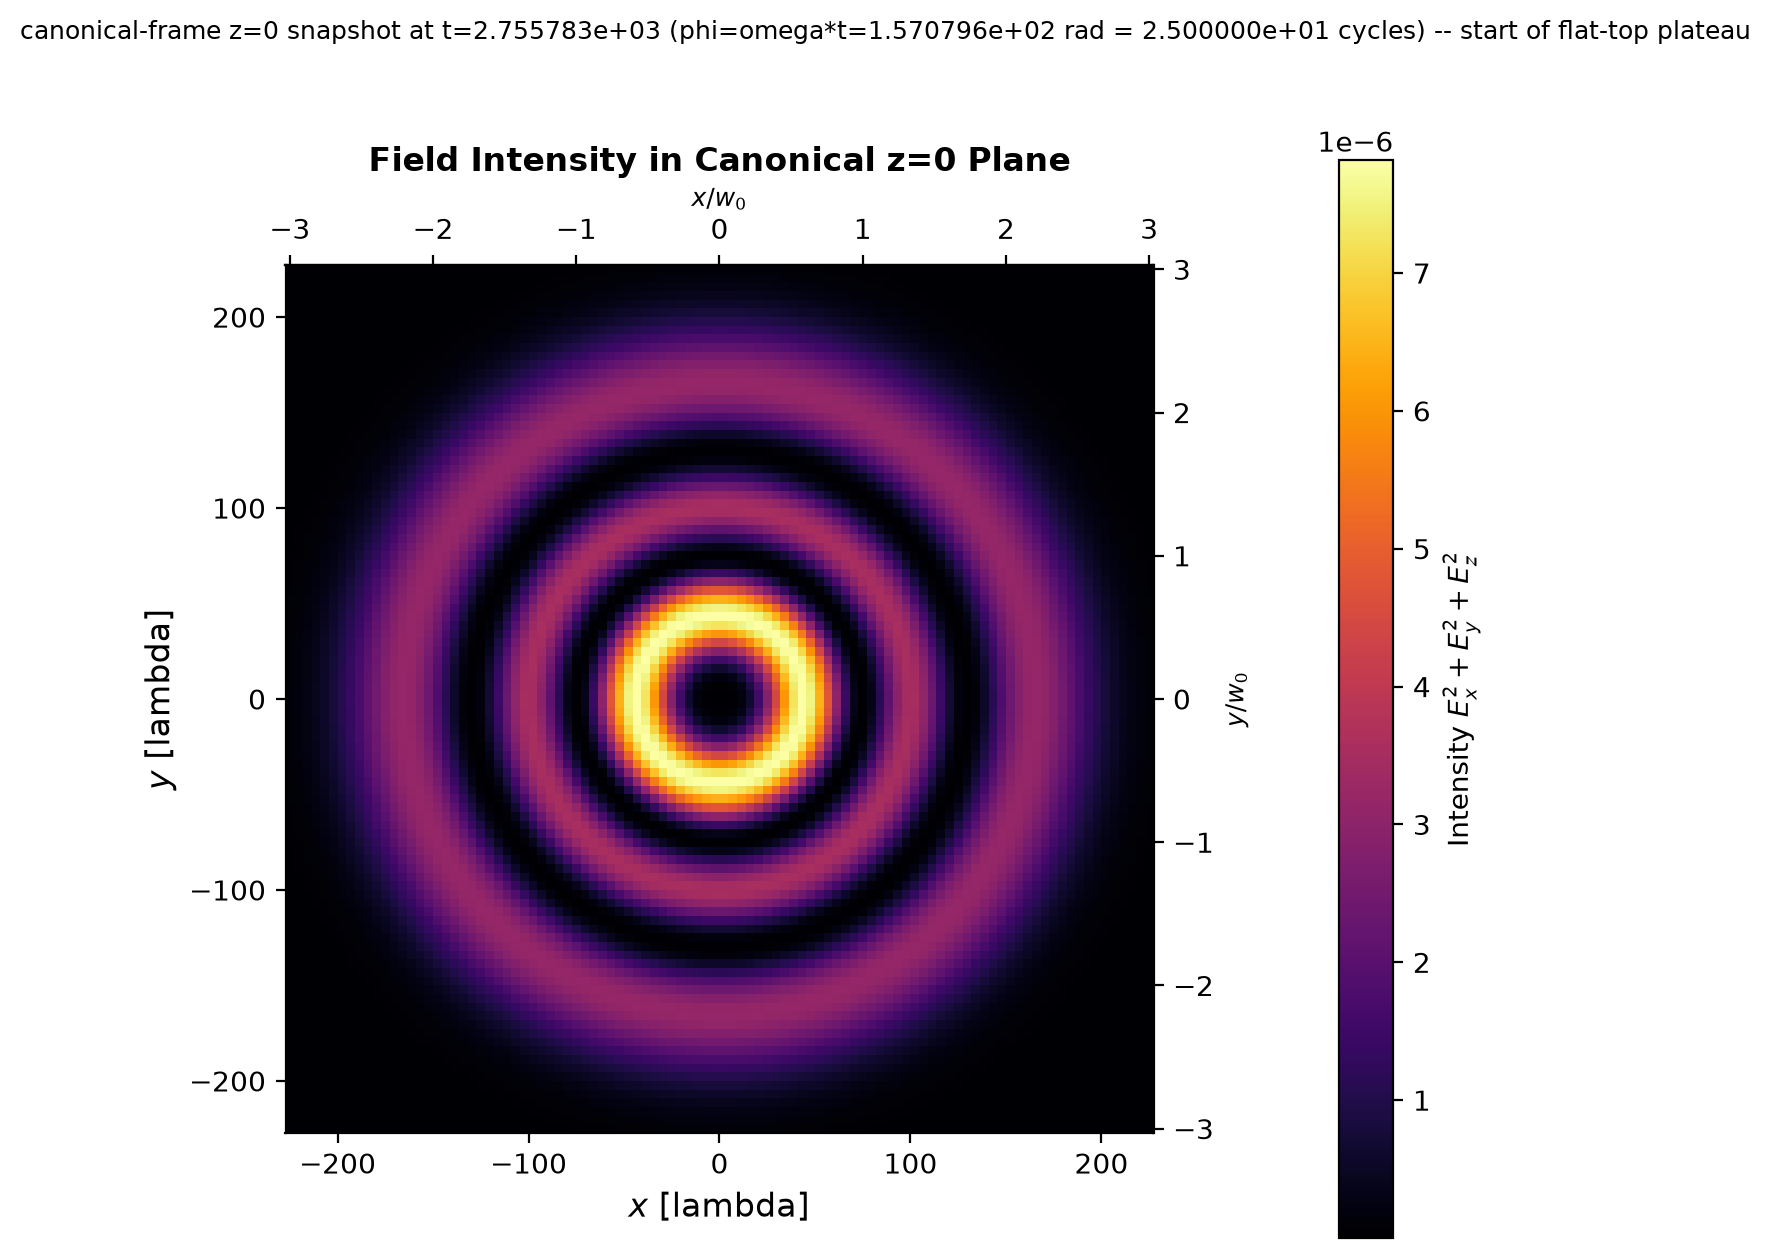
\includegraphics[height=0.62\textheight]{figs/laser_field_heatmap_z0_plot.png}
\end{frame}
\section{Equations of motion for the charged particle in the electromagnetic field}
\begin{frame}{Equations of motion for the charged particle in the electromagnetic field}
  \theorylabel{The Faraday tensor of the electromagnetic field}
  \begin{align*}
    F^{\mu\nu}(x)=\left(
      \begin{array}{cccc}0&-\tilde E_x/c& -\tilde E_y/c& -\tilde E_z/c\\\tilde E_x/c&0&-\tilde B_z&\tilde B_y\\\tilde E_y/c&\tilde B_z&0&-\tilde B_x\\\tilde E_z/c&-\tilde B_y&\tilde B_x&0
    \end{array}\right)
  \end{align*}

  \theorylabel{The covariant equations of motion}

  \begin{equationpanel}
    \begin{align*}
      & \frac{dx^{\mu}}{d\tau} = \frac{p^{\mu}}m, \qquad \frac{dp^\mu}{d\tau} = \frac{q}{m} F^{\mu\nu}(x)p_\nu,
    \end{align*}
  \end{equationpanel}

\end{frame}

\begin{frame}{Equations of motion for the charged particle in the electromagnetic field}

  Time dependence of the momentum for 10 electrons in the initial beam

  \begin{center}
    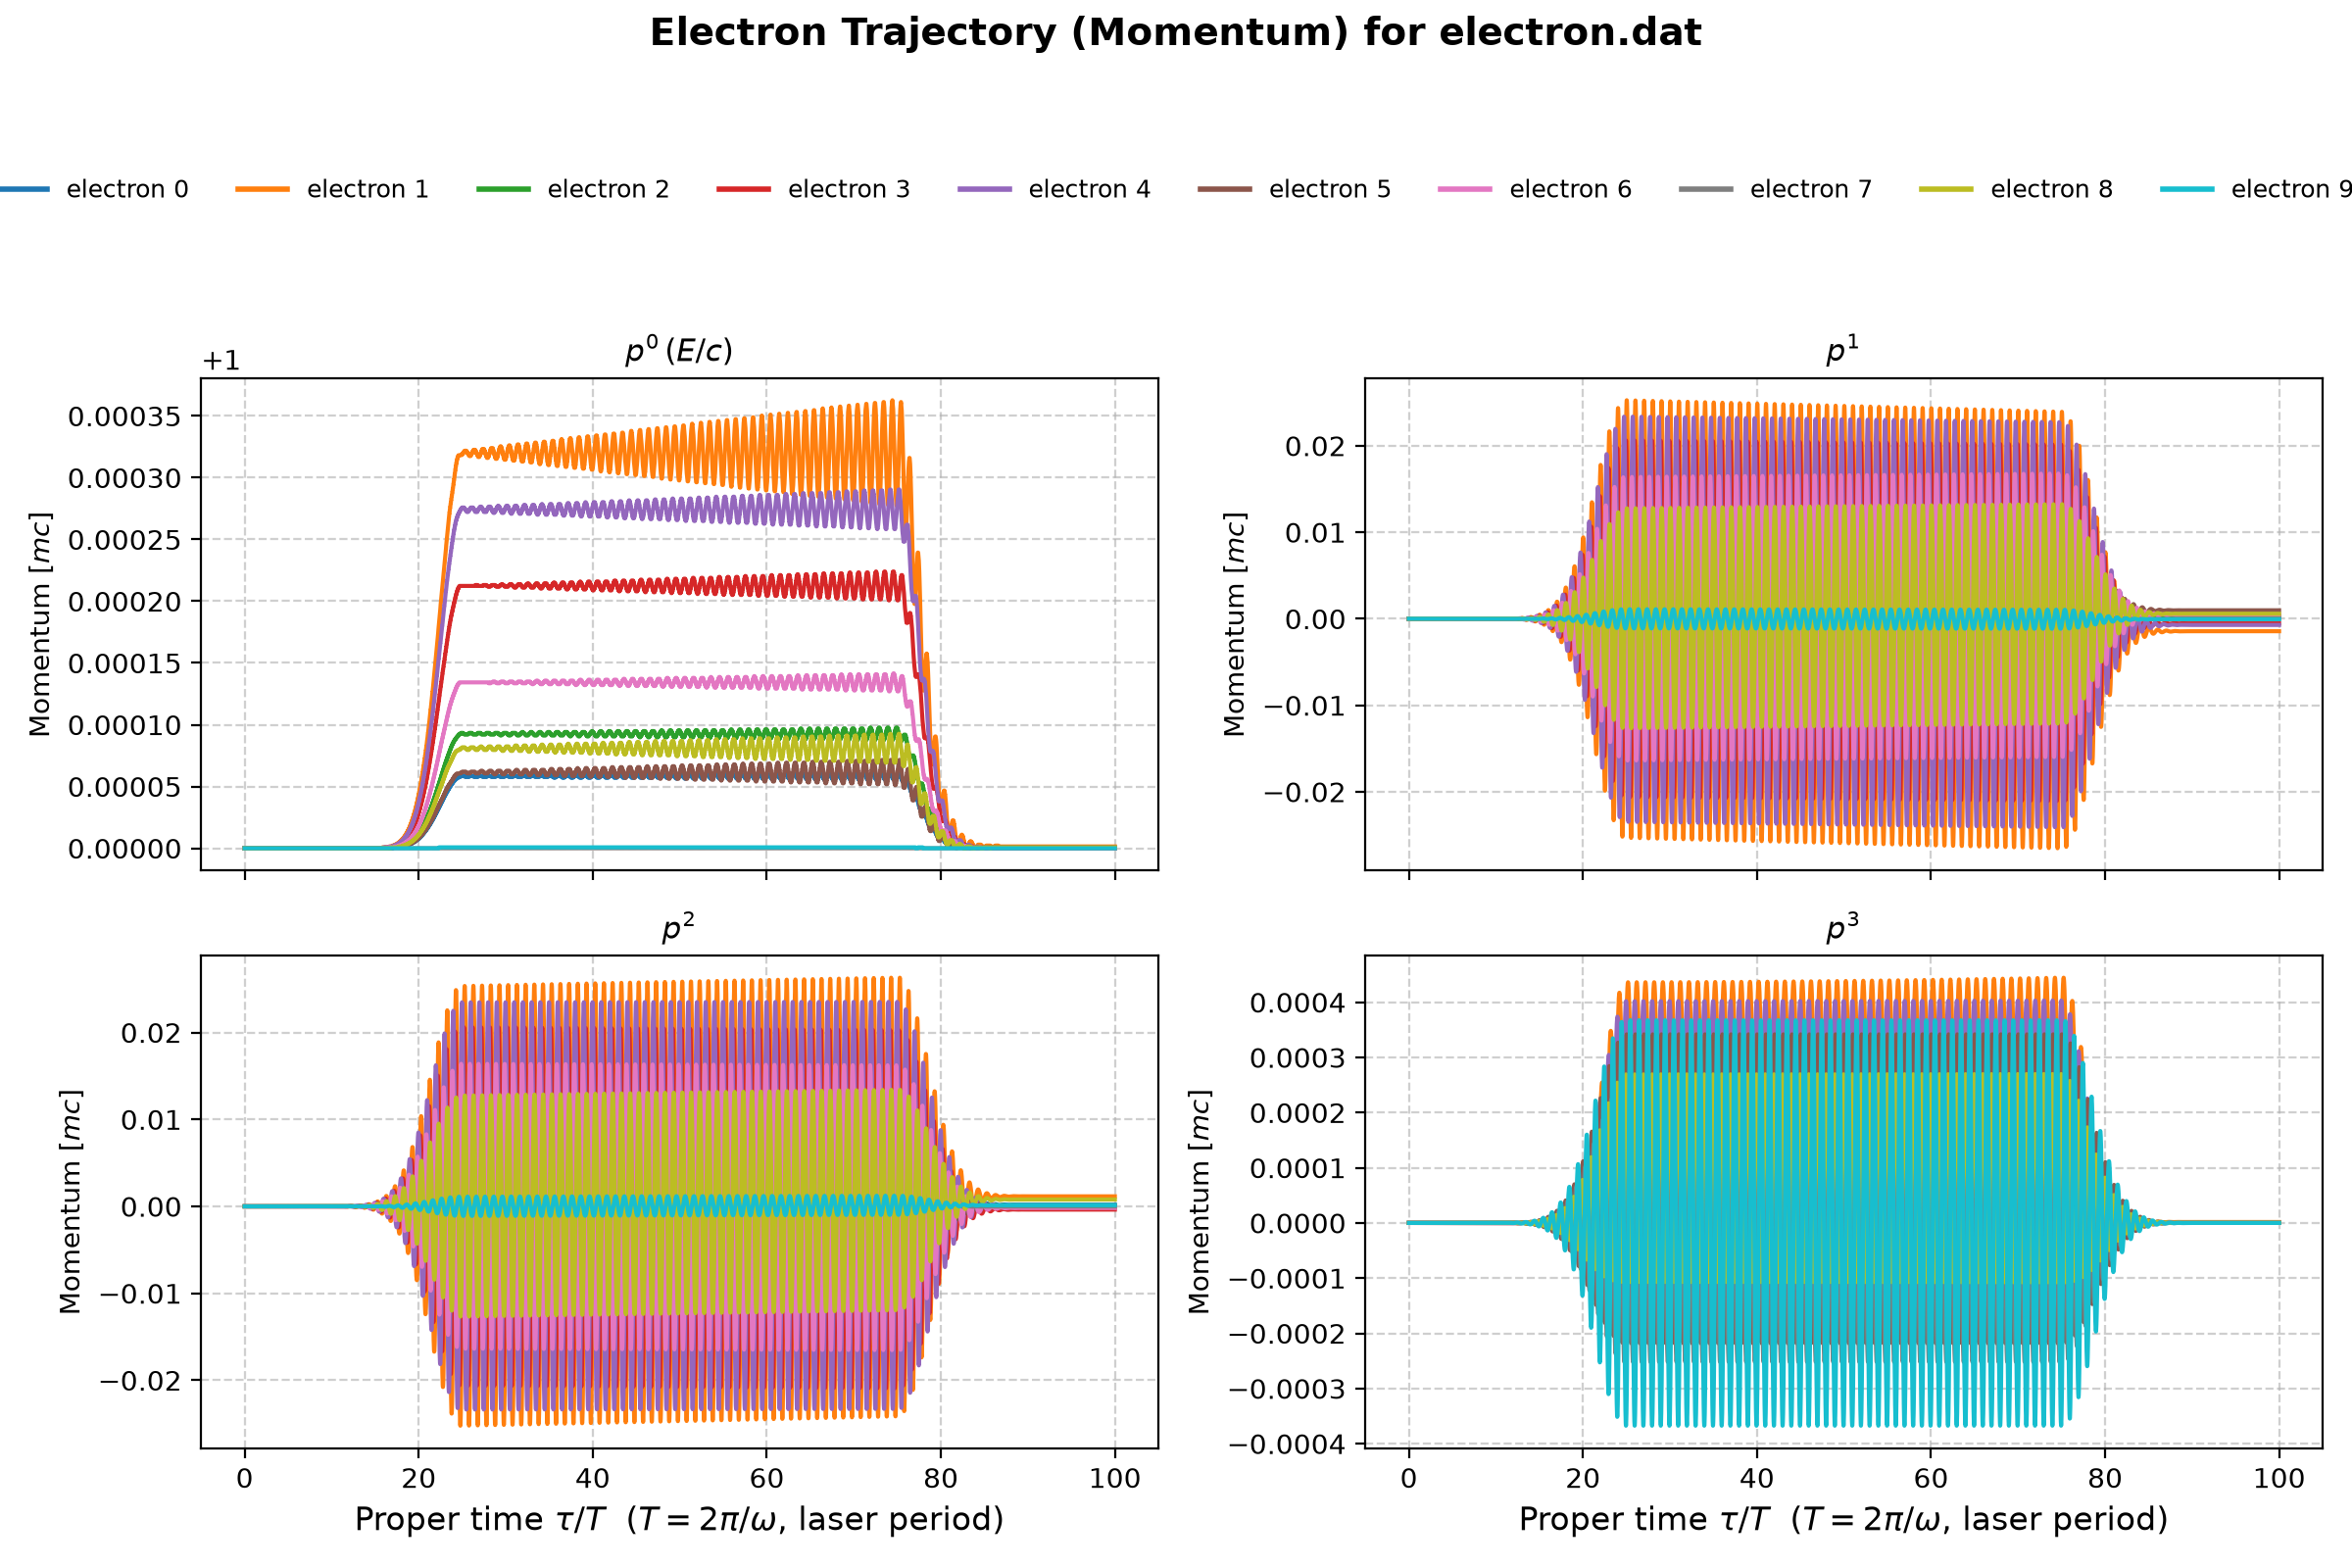
\includegraphics[scale = 0.3]{figs/electron_momentum_profile.png}
  \end{center}

\end{frame}

\section{The non-linear Thomson scattering}
\begin{frame}{The non-linear Thomson scattering}
  \framesubtitle{The temporal domain}
  The Lienard Wiechert potentials of the emitted field are
  \begin{align*}
    A(x) & =\frac{ec\mu_0}{4\pi}\frac{u(\tau_r)}{u(\tau_r)\cdot(x_0-r_0(\tau_r))}=\frac{e}{4\pi\epsilon_0c}\frac{u(\tau_r)}{u(\tau_r)\cdot(x_0-r_0(\tau_r))}
  \end{align*}
  and there are two forms of the coresponding Faraday tensor
  \begin{align*}
    F^{\alpha\beta}(x) & =\partial^{\alpha}A^{\beta}(x)-\partial^{\beta}A^{\alpha}(x) ={\frac{e}{4\pi\epsilon_0c}\frac{(u\cdot R_0)(R_0^{\alpha}w^{\beta}-R_0^{\beta}w^{\alpha})-((w\cdot R_0)-c^2)(R_0^{\alpha}u^{\beta}-R_0^{\beta}u^{\alpha})}{(u\cdot R_0)^3}  \vline}_{\tau=\tau_r}\\
    &={\frac{e}{4\pi\epsilon_0c}\frac1{(u\cdot R_0)}\frac{d}{d\tau}\left[\frac{R_0^{\alpha}u^{\beta}-R_0^{\beta}u^{\alpha}}{(R_0\cdot u)}\right]\vline}_{\tau=\tau_r}
  \end{align*}
  with $\tau_r$ the retarded proper time. In the previous equation the following notations have been used
  \begin{itemize}
    \item $\boldsymbol{\mathfrak R}_0$ - the particle initial position (not the origin), ${\bf x}$ - the observation point, $r(\tau)$ - the particle trajectory, $R_0(\tau;t) = (ct-{r}^0_0(\tau), {\bf r}(\tau)-{\boldsymbol{\mathfrak R}}_0)$ (the trajectory relative to the initial position)
    \item $u(\tau)$ - the particle 4-velocity, $w(\tau)$ the particle 4 acceleration
    \item the proper time is defined as the solution of the equation $R_0(\tau_r;t)\cdot R_{0}{(\tau_r;t)}=0$
  \end{itemize}

\end{frame}

\begin{frame}{The non-linear Thomson scattering}
  \framesubtitle{The frequency domain}
  The Fourier transform of the Faraday tensor, after the change of variable from the time the lab frame $t$ to the retarded time $\tau_r$
  \begin{align*}
    F^{\alpha\beta}(ck,{\bf x})=\frac1{2\pi}\frac{e}{4\pi\epsilon_0c^2|{\bf R}_0|}\int\limits_{-\infty}^{\infty}d\tau &e^{ik\left(r_0^0(\tau)+|{\bf x}_0-{\bf r}_0(\tau)|\right)}\frac{(u\cdot R_0)(R_0^{\alpha}w^{\beta}-R_0^{\beta}w^{\alpha})
    -((w\cdot R_0)-c^2)(R_0^{\alpha}u^{\beta}-R_0^{\beta}u^{\alpha})}
    {(u\cdot R_0)^2}\label{eq:F-direct-corrected}
  \end{align*}
  The formula requires storing the acceleration of the particle at any time. An equivalent approach starts from
  \begin{align*}
    F^{\alpha\beta}=(ct, {\bf x})= {\frac{e}{4\pi\epsilon_0c}\frac1{(u\cdot R_0)}\frac{d}{d\tau}\left[\frac{R_0^{\alpha}u^{\beta}-R_0^{\beta}u^{\alpha}}{(R_0\cdot u)}\right]\vline}_{\tau=\tau_r}
  \end{align*}
  and used an integration by parts with the results
  \begin{align*}
    F_s^{\alpha\beta}(ck,{\bf x}) & =\frac1{2\pi}\frac{e}{4\pi\epsilon_0|{\bf R}_0|^2}\int\limits_{-\infty}^{\infty}d\tau e^{ik\left(r_0^0+|{\bf R}_0|\right)}\frac{(n_{R_0}^{\alpha}u^{\beta}-n_{R_0}^{\beta}u^{\alpha})}
    {(u\cdot n_{R_0})^2}
  \end{align*}
  \theorylabel{The boundary term must be kept in the numerical calculation}

  The standard split is  $F_{total}=F_{long}+F_{short}$; For the typical case (the screen at macroscopic distances from the electron beam) the short component is completely irrelevant

\end{frame}

\begin{frame}{The non-linear Thomson scattering}
  \framesubtitle{Numerical example: the direct formula}

  {\tiny
    $a_0=0.1$ (dimensionless), $\omega_l=0.057$ a.u.; electrons initially at rest;
    $N_{\mathrm{electron}}=16384$.\\
    Typical CPU time: $7.8\,\mu\mathrm{s}$ per electron, screen point and cycle.
    Only results for the fundamental harmonic are presented.
  \par}
  {\par\centering
    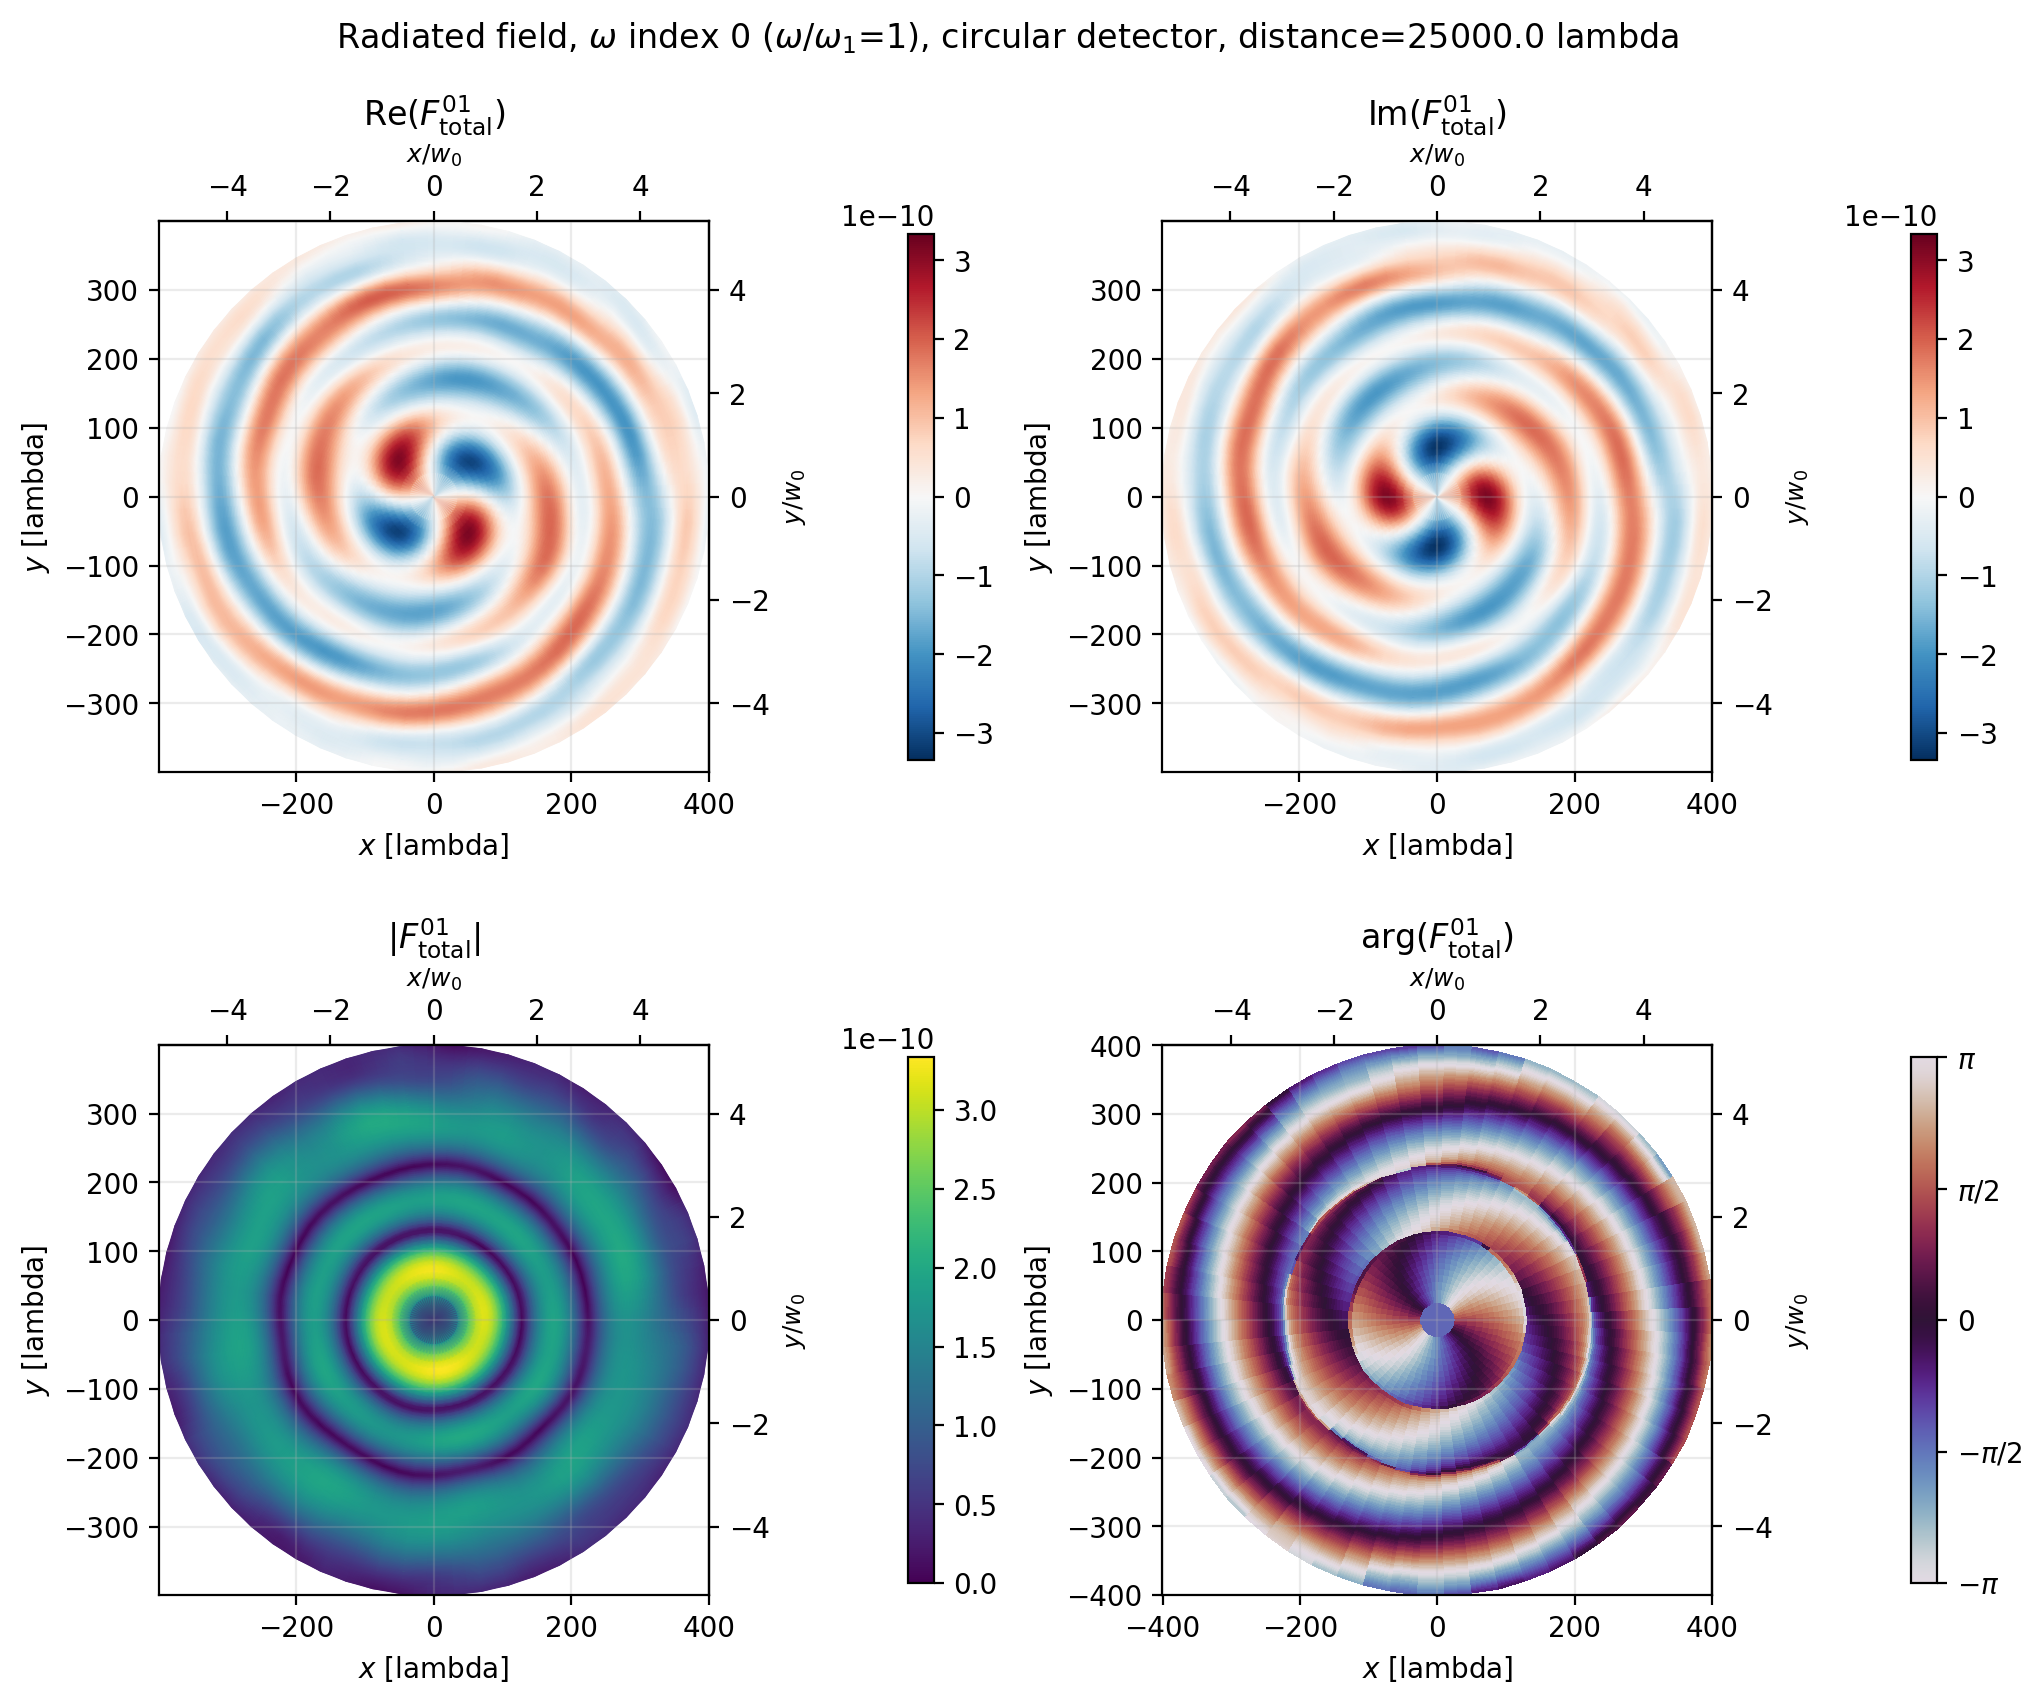
\includegraphics[scale=0.25]{figs/radiation_field_total_F01_omega0.png} \hspace{0.5cm}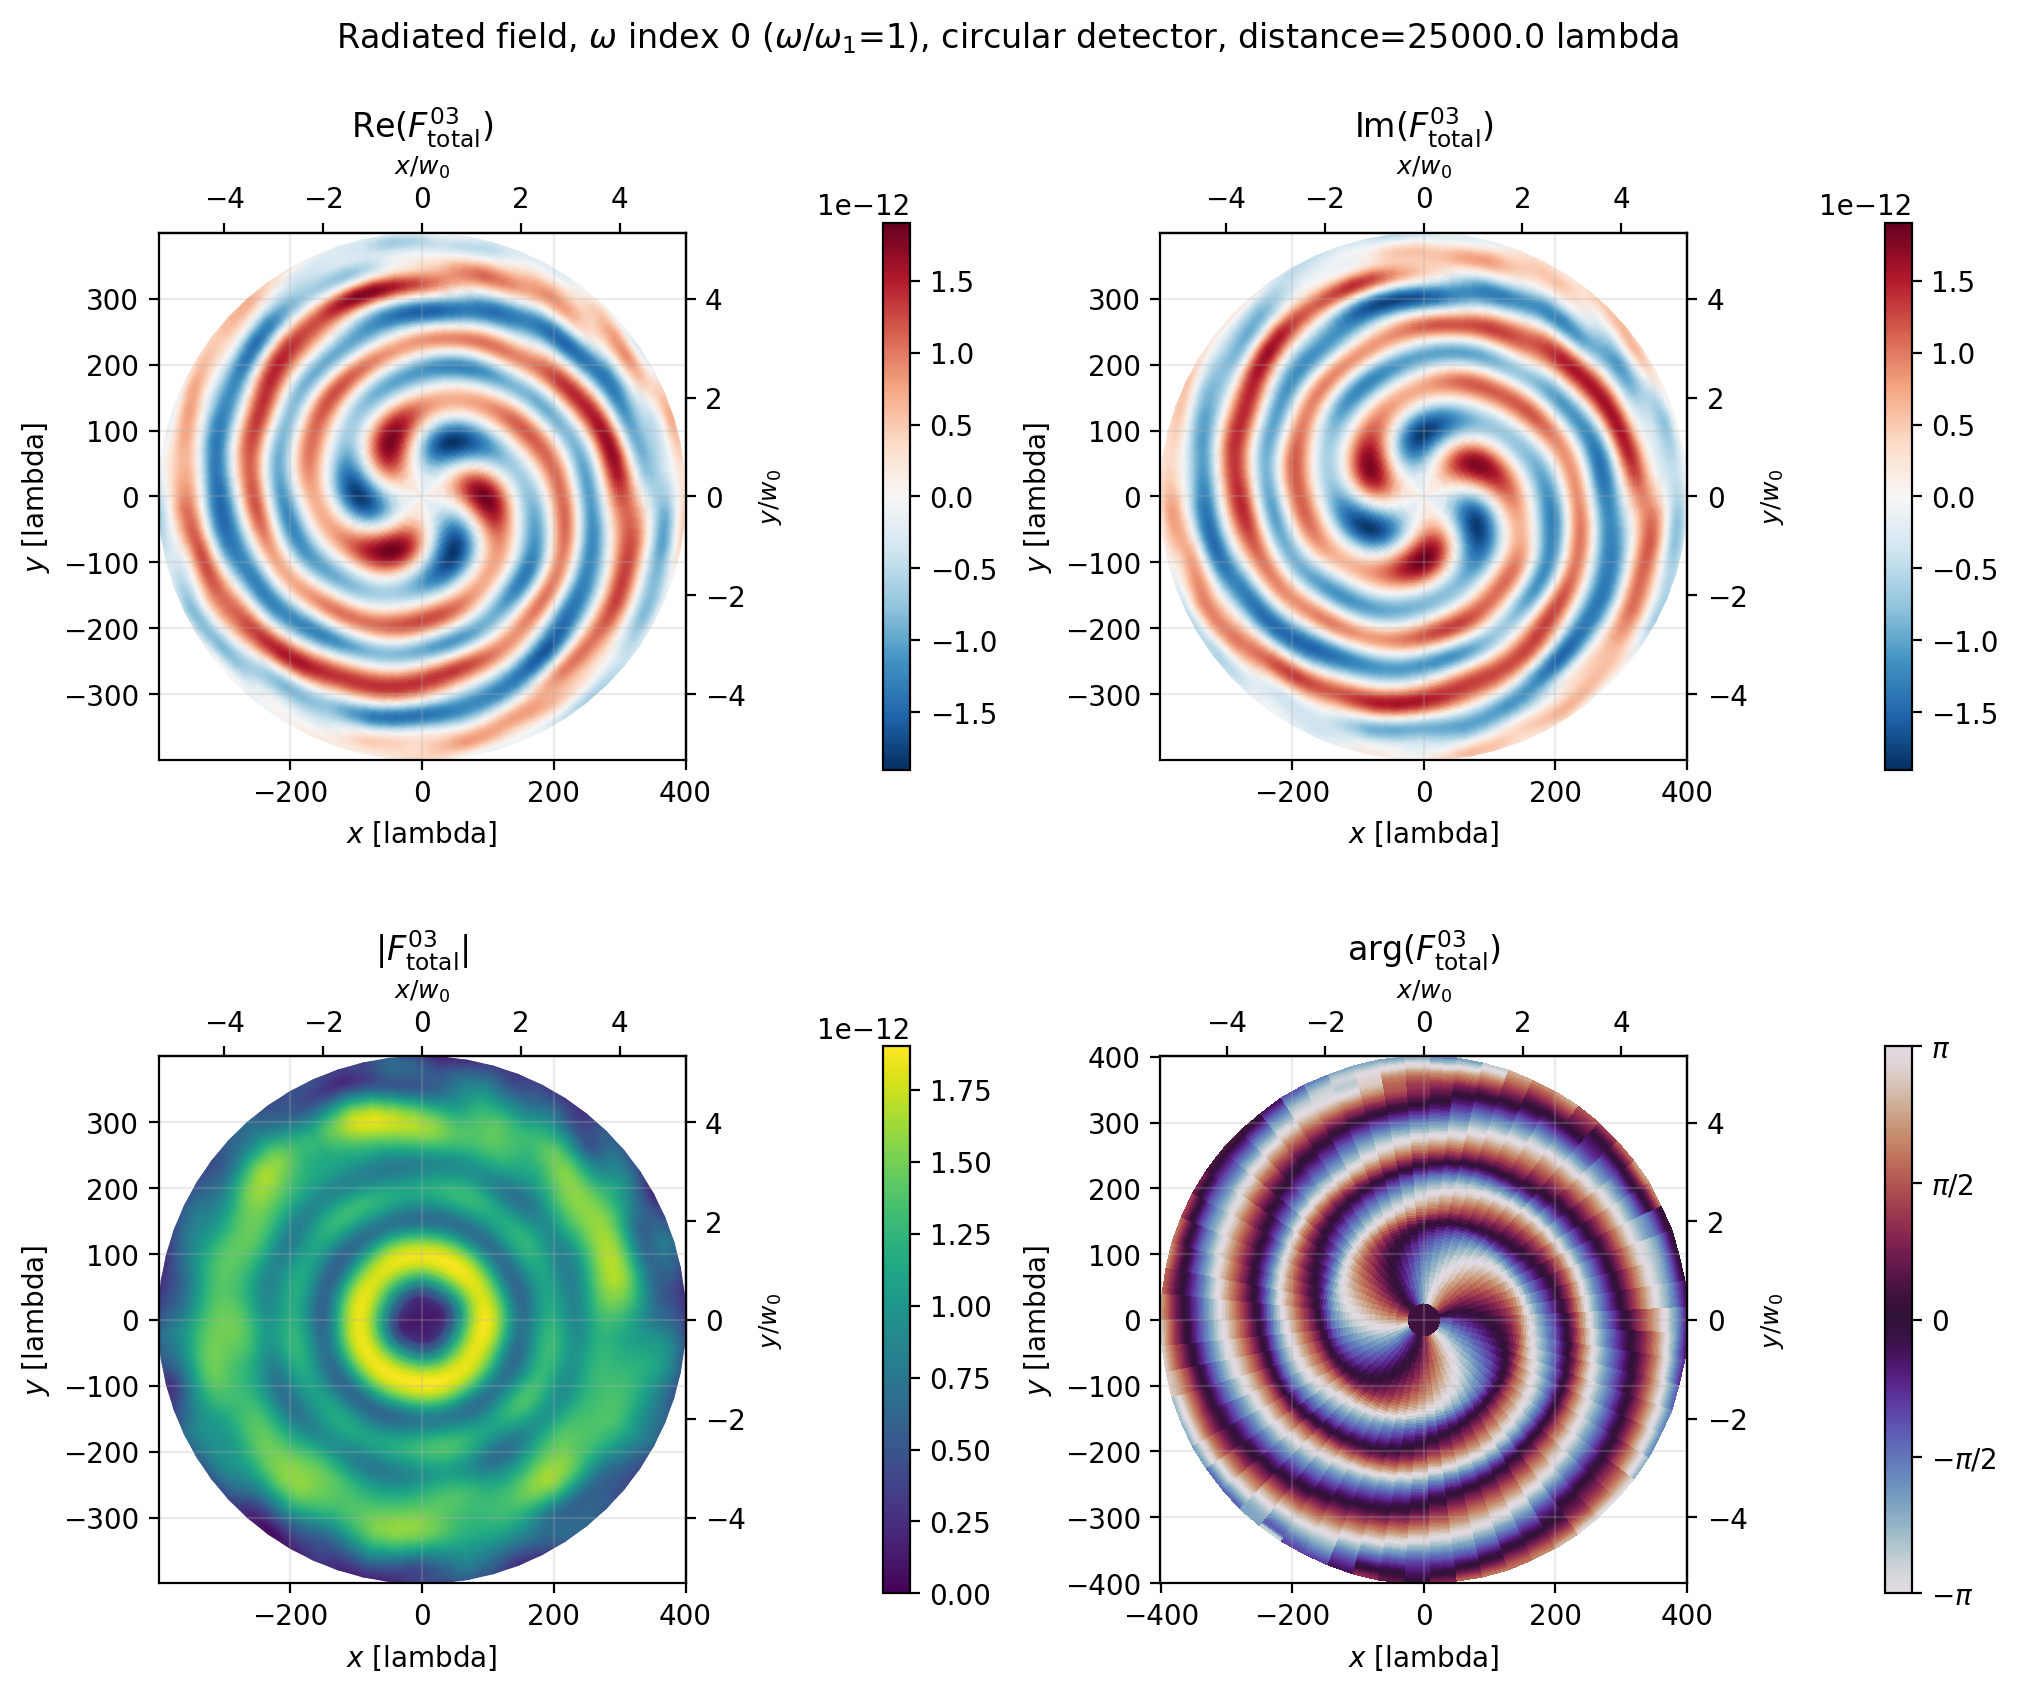
\includegraphics[scale=0.25]{figs/radiation_field_total_F03_omega0.png}
  \par}

  {\tiny Results obtained with the direct formula: $F^{01}\gg F^{03}$ (the transversality condition).\par}

\end{frame}

% Summary of FT_Faraday_tensor-direct_and_simplified_forms.md
\begin{frame}{The non-linear Thomson scattering}
  \framesubtitle{The frequency domain: two equivalent forms}
  \setlength{\abovedisplayskip}{3pt}
  \setlength{\belowdisplayskip}{3pt}
  For the same trajectory and observation point, define
  \begin{align*}
    R &= |{\bf x}_0-{\bf r}_0(\tau)|,\quad
    n=(1,({\bf x}_0-{\bf r}_0)/R),\quad
    \Phi=r_0^0+R,\quad k=\omega/c,\quad C=\frac{1}{2\pi}\frac{e}{4\pi\epsilon_0c^2},\\
    D &= u\cdot n,\quad
    A^{\alpha\beta}=n^\alpha u^\beta-n^\beta u^\alpha,\quad
    B^{\alpha\beta}=n^\alpha w^\beta-n^\beta w^\alpha,
    \qquad \frac{dt}{d\tau}=\frac{D}{c}.
  \end{align*}
  \theorylabel{The direct form} (trajectory, velocity and acceleration)
  \begin{align*}
    F_{\mathrm{direct}}^{\alpha\beta}
    &=C\int_{\tau_{\min}}^{\tau_{\max}}d\tau\,e^{ik\Phi}
    \left[\frac{D B^{\alpha\beta}-(w\cdot n)A^{\alpha\beta}}{R D^2}
    +\frac{c^2 A^{\alpha\beta}}{R^2 D^2}\right].
  \end{align*}
  \theorylabel{The simplified form} (integration by parts; no explicit acceleration)
  \begin{align*}
    F_{\mathrm{simplified}}^{\alpha\beta}
    &=C\int_{\tau_{\min}}^{\tau_{\max}}d\tau\,e^{ik\Phi}
    \left[-\frac{ikD}{R}-\frac{{\bf n}\cdot{\bf u}}{R^2}\right]
    \frac{A^{\alpha\beta}}{D}+F_b^{\alpha\beta},\\
    F_b^{\alpha\beta}
    &=C\left[\frac{e^{ik\Phi}}{R}\frac{A^{\alpha\beta}}{D}\right]_{\tau_{\min}}^{\tau_{\max}}.
  \end{align*}
  \begin{itemize}
    \item Keep the boundary term for a finite trajectory window. Compare the \alert{total fields} in all six independent components; the separate long- and short-range terms need not agree.
  \end{itemize}
\end{frame}

\begin{frame}{The non-linear Thomson scattering}
  \framesubtitle{Numerical example: the direct formula}

  {\par\centering
    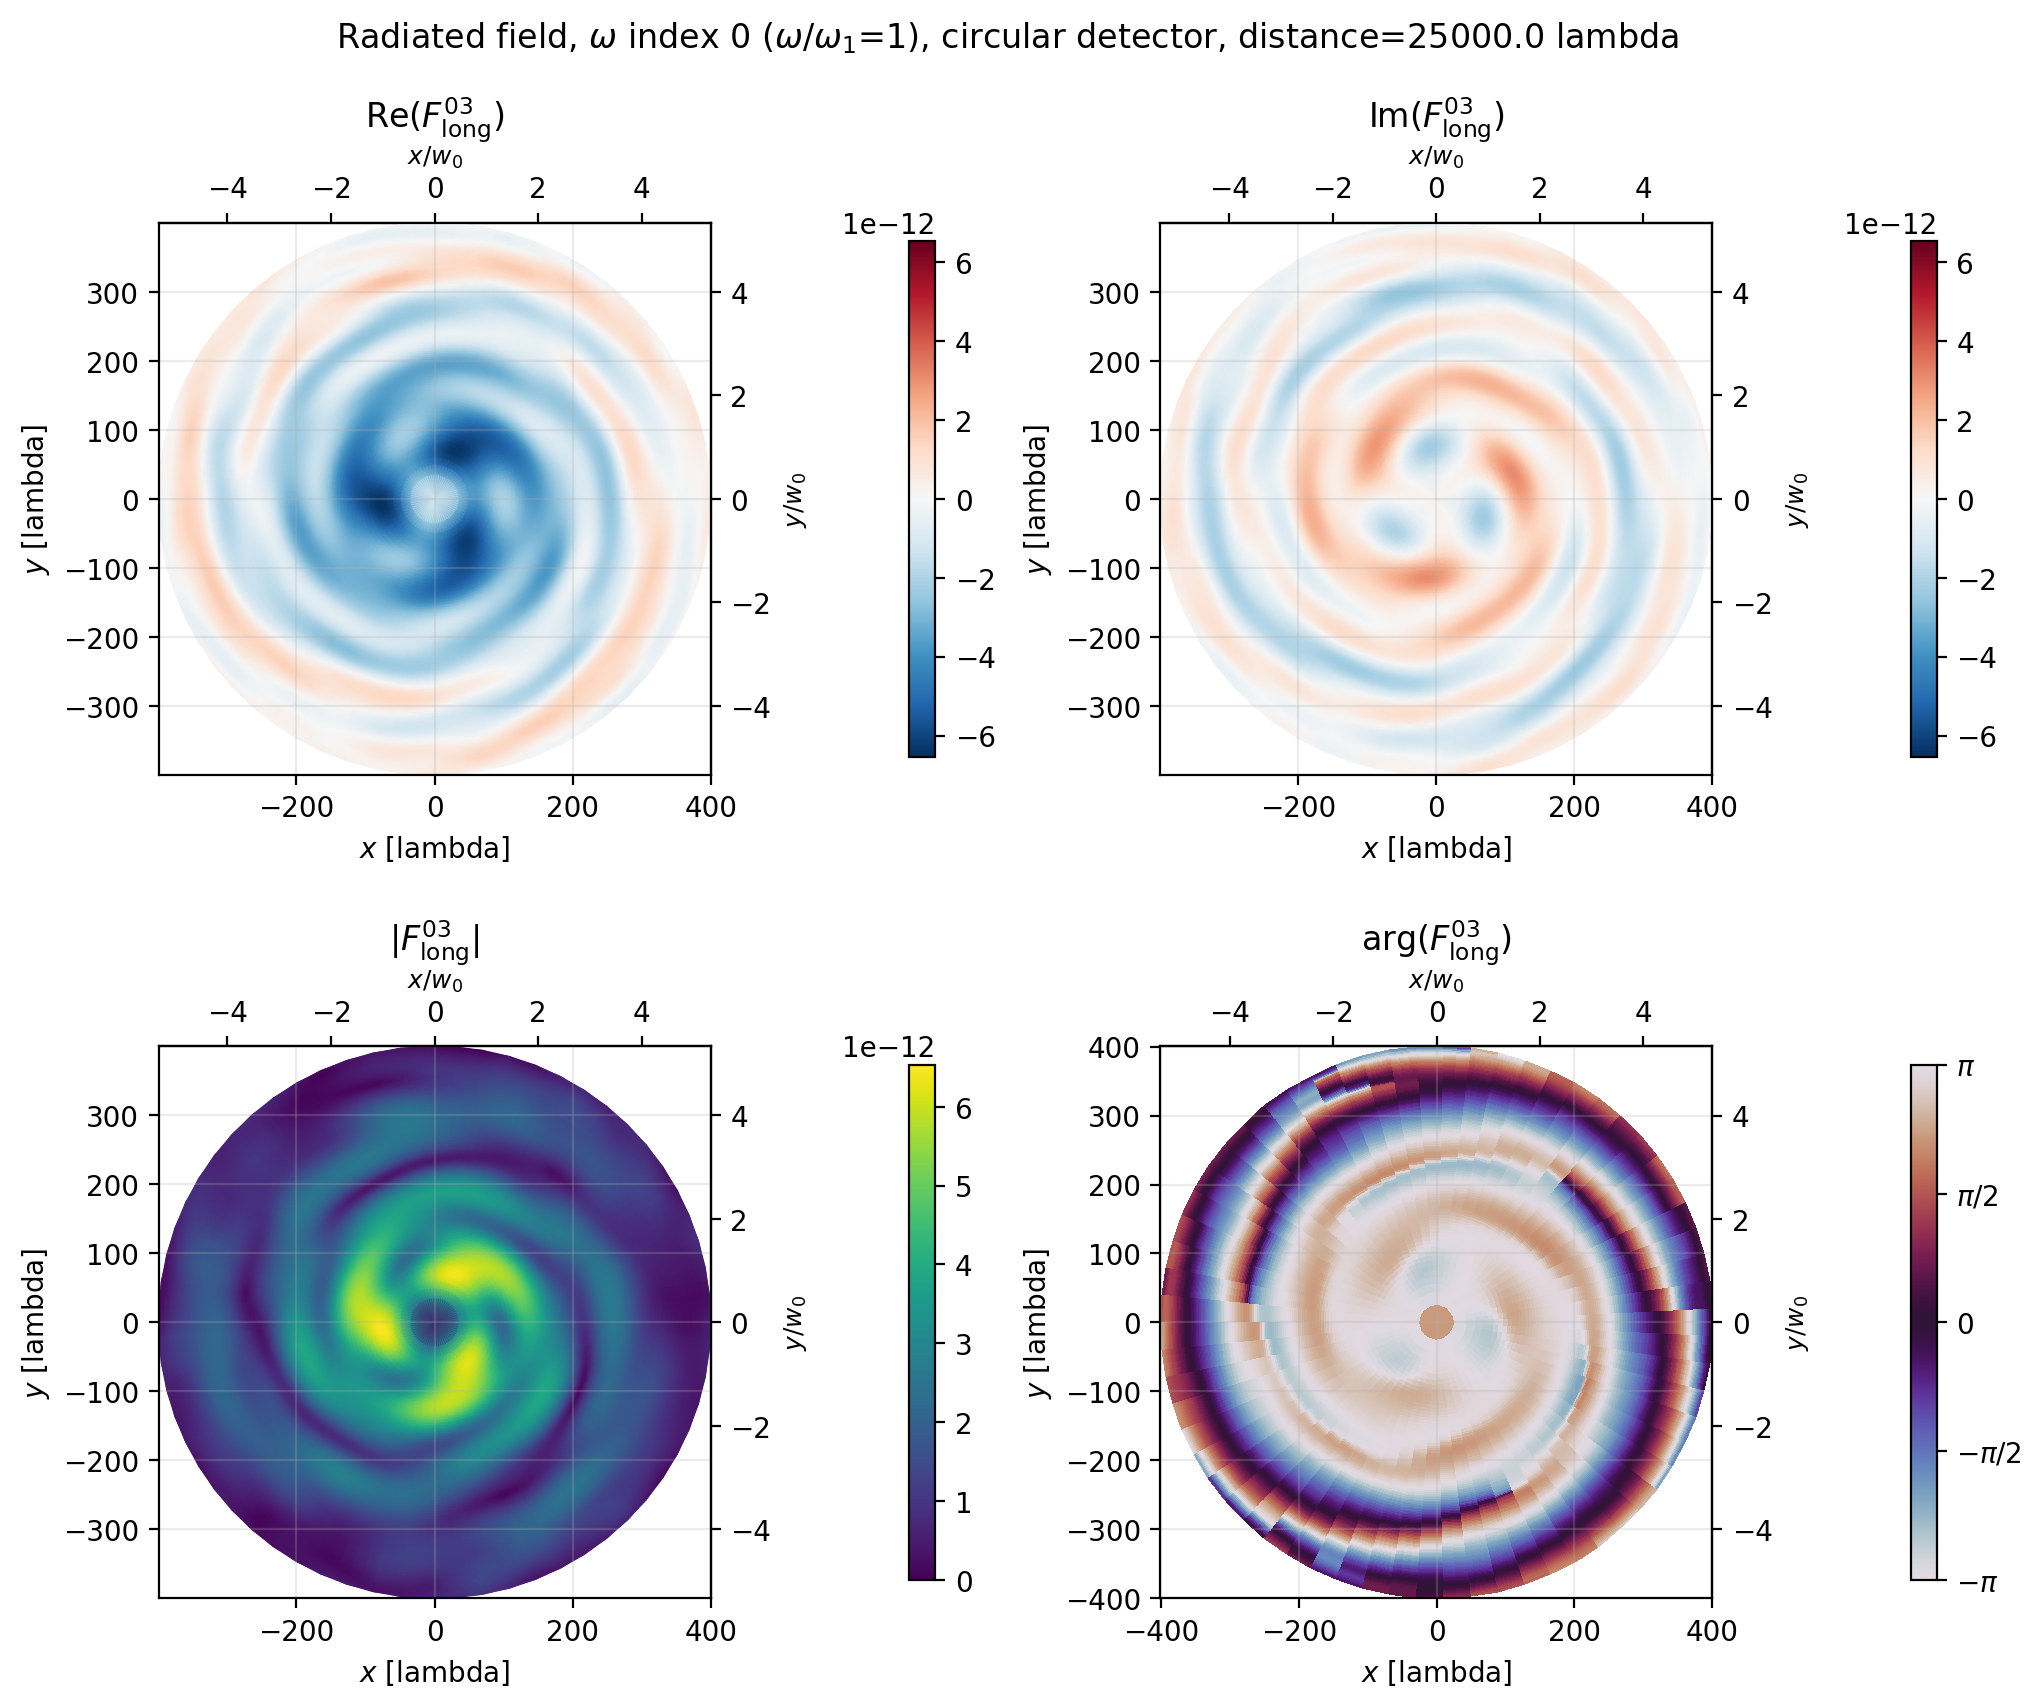
\includegraphics[scale=0.25]{figs/radiation_field_long_F03_omega0.png} \hspace{0.5cm}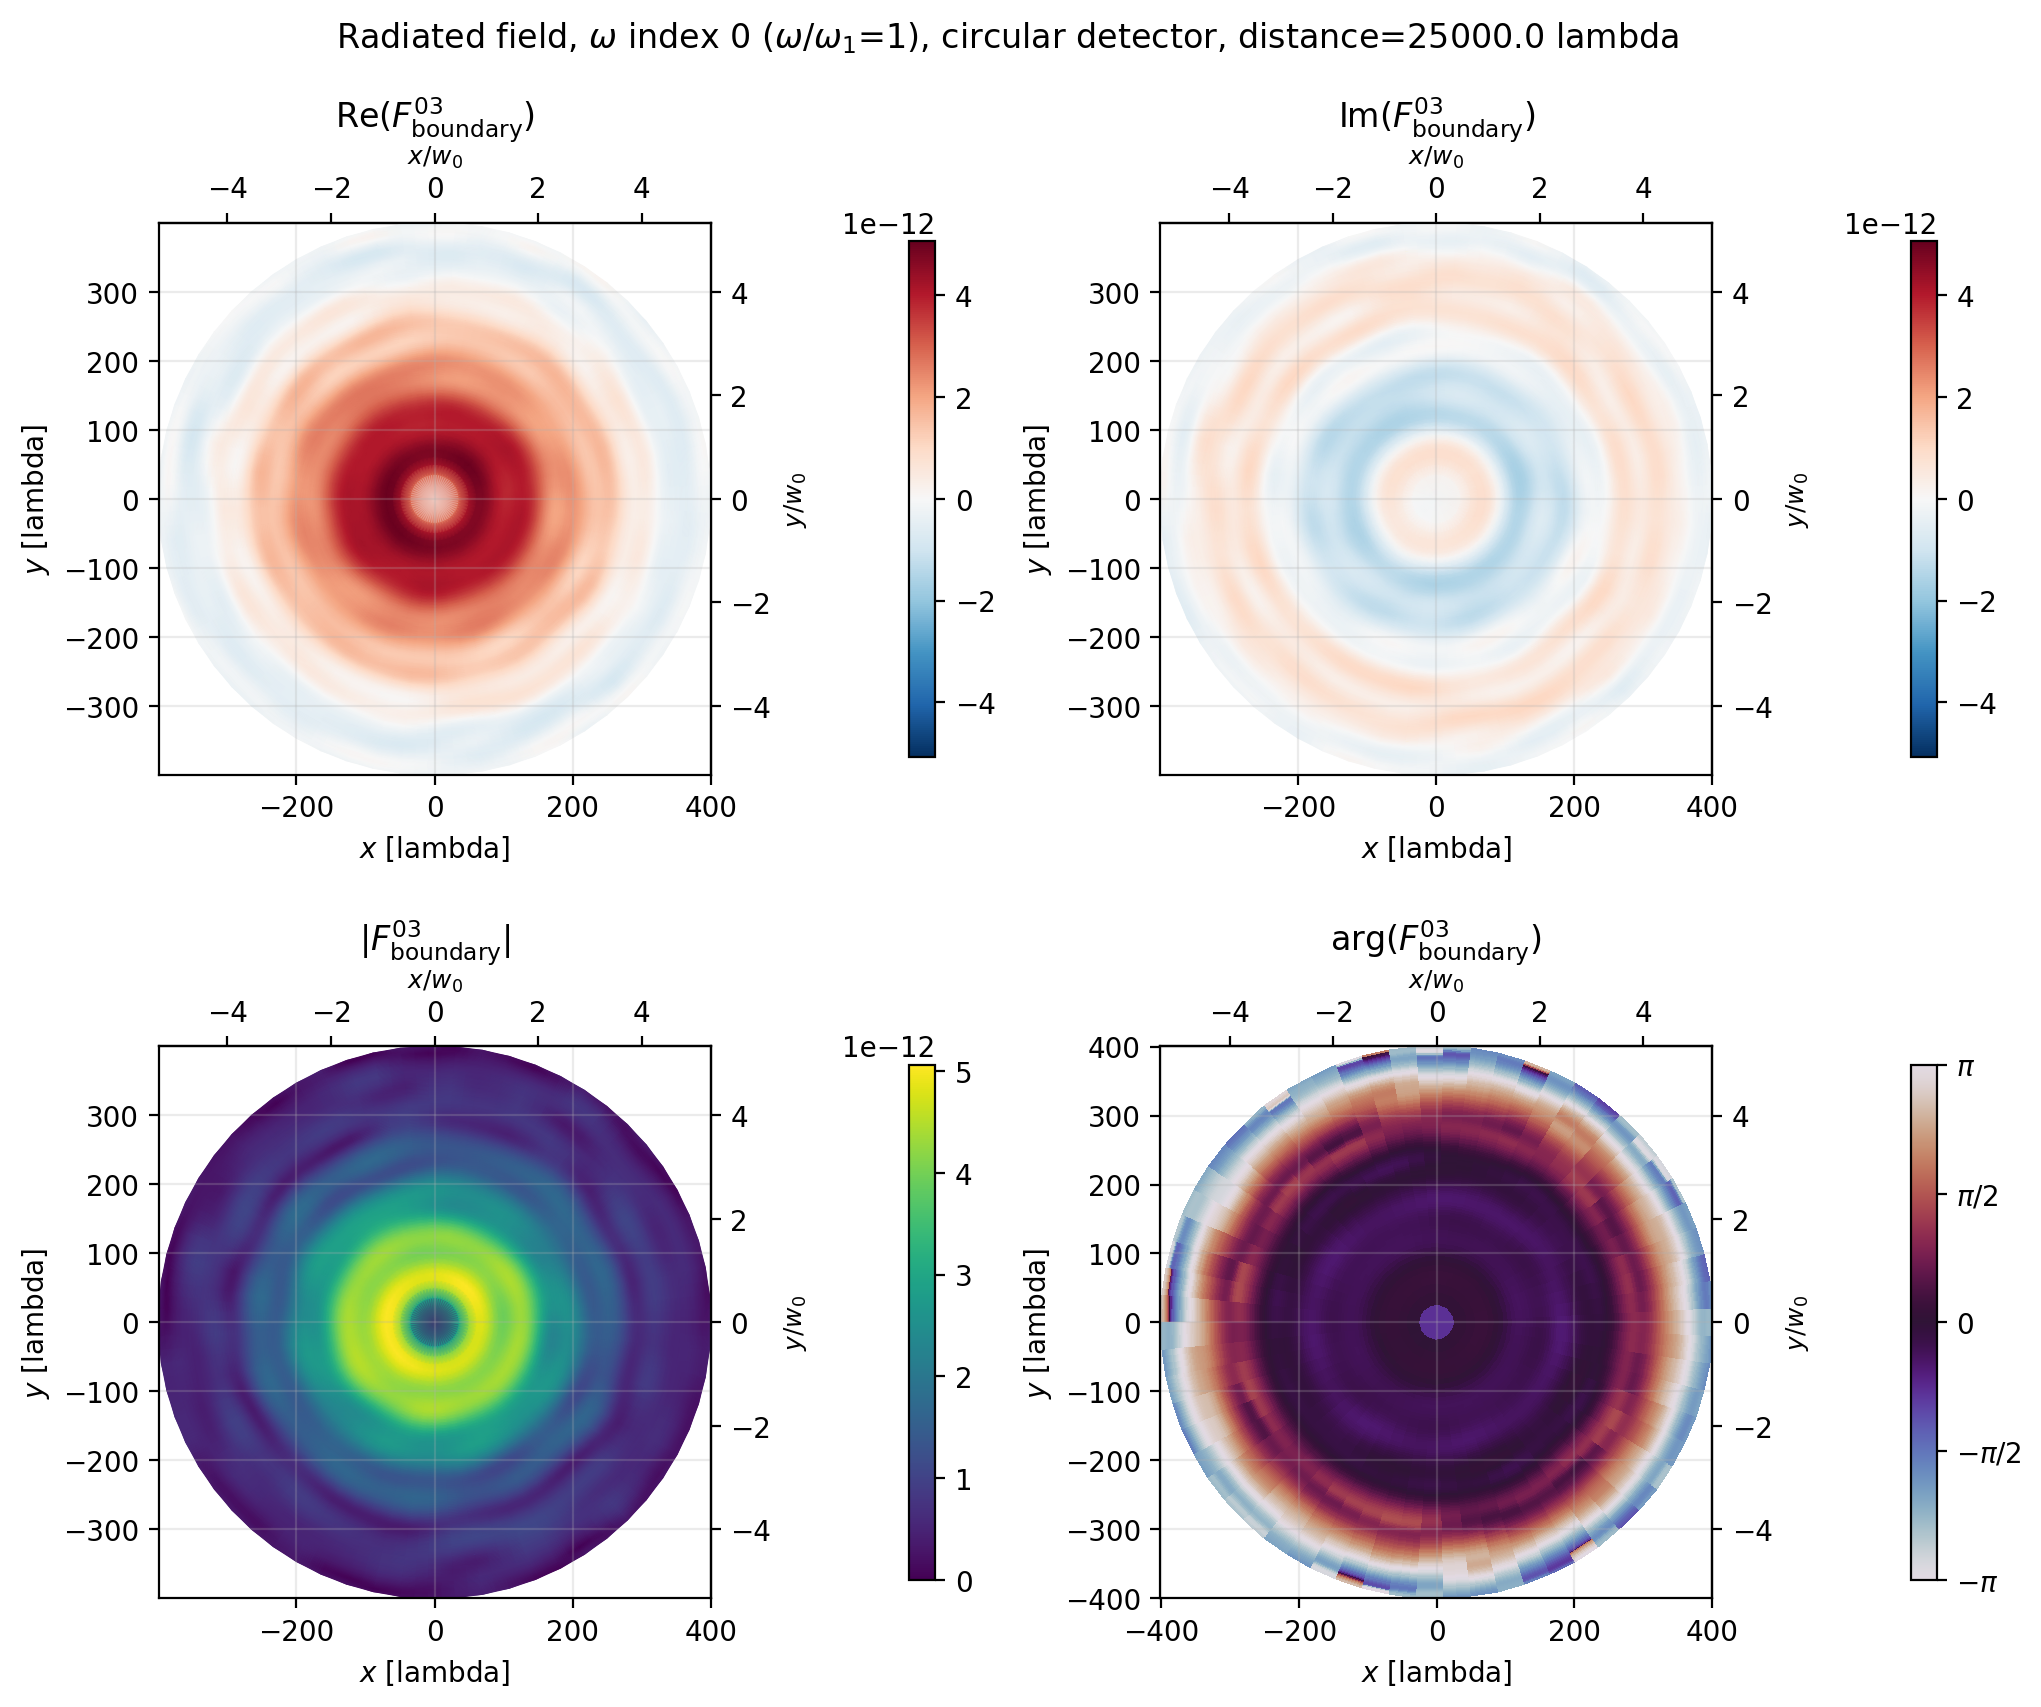
\includegraphics[scale=0.25]{figs/radiation_field_boundary_F03_omega0.png}
  \par}

  \vspace{-3pt}
  \begin{validationtest}{1}{Agreement of the two forms}
    \tiny
    $F^{03}_{\text{long}}+F^{03}_{\text{boundary}}\simeq F^{03}_{\text{direct}}$
    to high numerical accuracy. The neglected $F^{03}_{\text{short}}$ is about eight orders of magnitude smaller.
  \end{validationtest}

\end{frame}

\section{The calculation of the observables of the field}
\begin{frame}{The calculation of the observables of the field}
  \framesubtitle{Fourier amplitudes and energy observables}
  \setlength{\abovedisplayskip}{3pt}
  \setlength{\belowdisplayskip}{3pt}
  At each observation point, the complex Faraday tensor gives
  \begin{align*}
    \tilde{\bf E}&=c(F^{10},F^{20},F^{30}),\qquad
    \tilde{\bf B}=(F^{32},F^{13},F^{21}),\qquad
    \tilde{\bf A}=\frac{\tilde{\bf E}}{i\omega}\quad(\omega>0).
  \end{align*}
  The vector potential is taken in the radiation gauge. Using the spectral convention
  of the numerical results, the bilinear relation for real field components $a(t)$ and $b(t)$ is
  \begin{align*}
    \frac{d\langle ab\rangle}{d\omega}=2\Re[\tilde a\tilde b^*],\qquad \omega>0.
  \end{align*}
  \theorylabel{Spectral energy density and energy flux} along the detector normal
  \begin{equationpanel}
    \begin{align*}
      \frac{d u}{d\omega}
      &=\epsilon_0\left(|\tilde{\bf E}|^2+c^2|\tilde{\bf B}|^2\right),\\
      \frac{d P_z}{d\omega}
      &=2\epsilon_0c^2\Re\left[\tilde E_x\tilde B_y^*-\tilde E_y\tilde B_x^*\right].
    \end{align*}
  \end{equationpanel}
  For a transverse wave propagating along $+z$, $d P_z/d\omega=c\,d u/d\omega$.
\end{frame}

\begin{frame}{The calculation of the observables of the field}
  \framesubtitle{Numerical example: energy flux and energy density on the screen}
  {\par\centering
    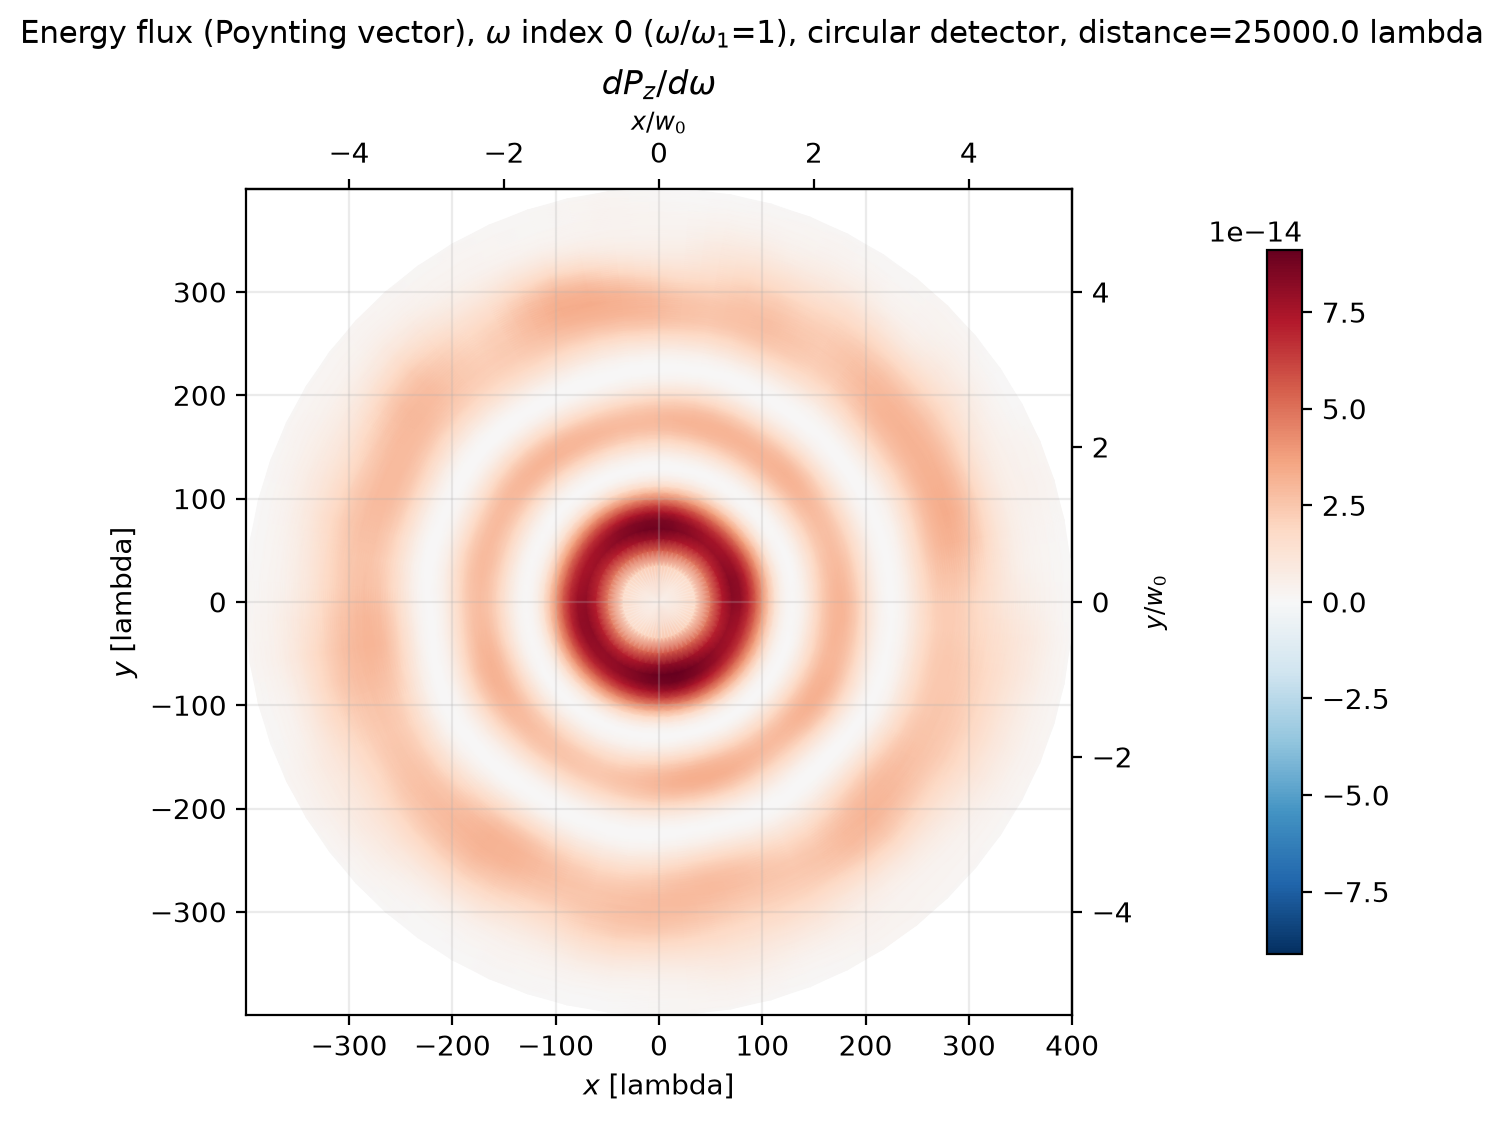
\includegraphics[scale=0.3]{figs/observable_energy_flux_omega0.png} \hspace{0.5cm}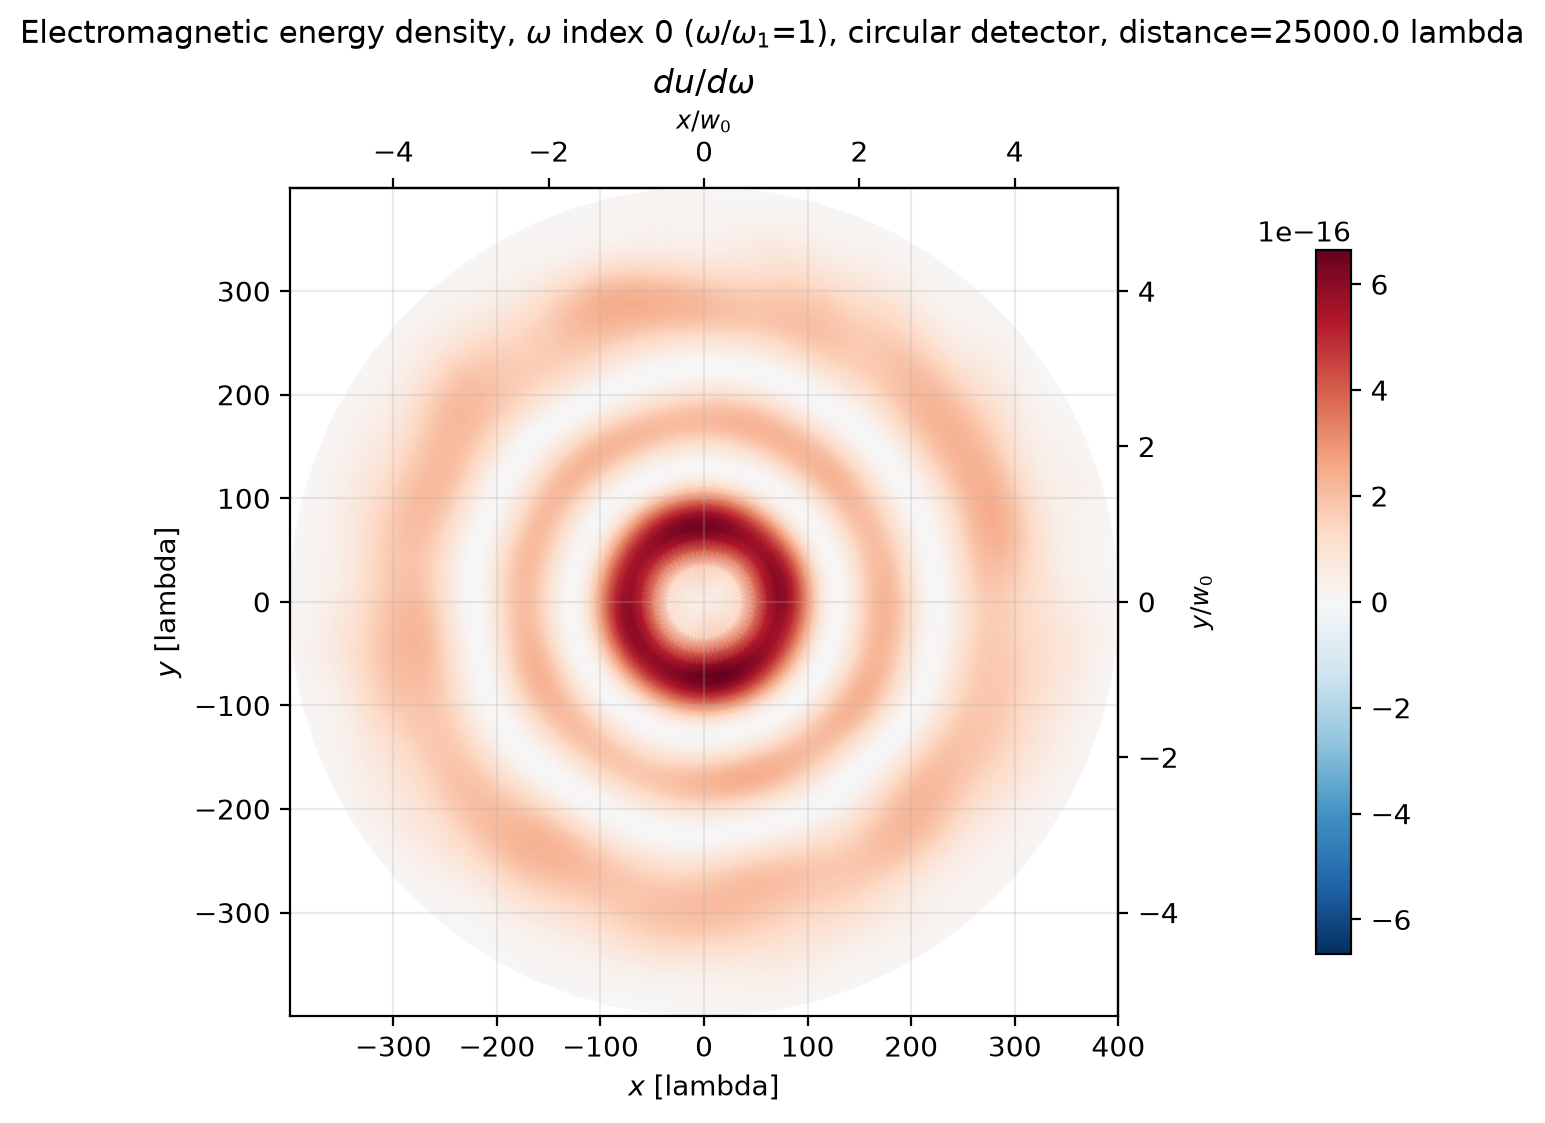
\includegraphics[scale=0.3]{figs/observable_energy_density_omega0.png}
  \par}

  \vspace{-2pt}
  \begin{validationtest}{2}{Energy transport at the speed of light}
    \tiny
    Screen-integrated spectral energy flux (left) / energy density (right):
    $\displaystyle
    \frac{\int_{\mathrm{screen}}dS\,d P_z/d\omega}
    {\int_{\mathrm{screen}}dS\,d u/d\omega}
    =1.370316\times10^{2}$ a.u.\\
    Reference: $c=1.37036\times10^{2}$ a.u.; relative deviation
    $\simeq3.21\times10^{-5}$ ($0.0032\%$).
  \end{validationtest}
\end{frame}
\begin{frame}{The calculation of the observables of the field}
  \framesubtitle{Spin and orbital angular momentum densities}
  \setlength{\parskip}{2pt}
  \setlength{\abovedisplayskip}{1pt}
  \setlength{\belowdisplayskip}{1pt}
  \setlength{\abovedisplayshortskip}{1pt}
  \setlength{\belowdisplayshortskip}{1pt}


  The canonical angular momentum densities in the radiation gauge are
  \begin{align*}
    {\boldsymbol{\cal S}}&=\epsilon_0{\bf E}\times{\bf A},\qquad
    {\boldsymbol{\cal L}}=\epsilon_0\sum_{i=x,y,z}E_i({\bf r}\times\boldsymbol\nabla)A_i.
  \end{align*}
  For the component along the beam axis, introduce the transverse operator
  \begin{align*}
    \hat L_z&=x\partial_y-y\partial_x=\partial_\phi,
    \qquad x=\rho\cos\phi,\quad y=\rho\sin\phi.
  \end{align*}
  Applying the bilinear spectral relation gives the \theorylabel{spin contribution}
  \begin{equationpanel}
    \begin{align*}
      \frac{d{\cal S}_z}{d\omega}
      &=\frac{4\epsilon_0}{\omega}\Im\left[\tilde E_x^*\tilde E_y\right],
    \end{align*}
  \end{equationpanel}
  and the \theorylabel{orbital contribution}, on Cartesian or polar detector grids,
  \begin{equationpanel}
    \begin{align*}
      \frac{d{\cal L}_z}{d\omega}
      &=\frac{2\epsilon_0}{\omega}\sum_{i=x,y,z}
      \Im\left[\tilde E_i^*\left(x\frac{\partial\tilde E_i}{\partial y}
      -y\frac{\partial\tilde E_i}{\partial x}\right)\right]\\
      &=\frac{2\epsilon_0}{\omega}\sum_{i=x,y,z}
      \Im\left[\tilde E_i^*\frac{\partial\tilde E_i}{\partial\phi}\right].
    \end{align*}
  \end{equationpanel}
  \theorylabel{Total angular momentum density:}\quad
  $\displaystyle\frac{d{\cal J}_z}{d\omega}
    =\frac{d{\cal S}_z}{d\omega}+\frac{d{\cal L}_z}{d\omega}$.
\end{frame}

\begin{frame}{The calculation of the observables of the field}
  \framesubtitle{Angular momentum fluxes through the detector}
  \setlength{\abovedisplayskip}{2pt}
  \setlength{\belowdisplayskip}{2pt}
  In vacuum, the spin and orbital densities satisfy the continuity equations
  \begin{align*}
    \partial_t{\cal S}_i+\partial_j\Sigma_{ij}=0,\qquad
    \partial_t{\cal L}_i+\partial_j\Lambda_{ij}=0.
  \end{align*}
  The fluxes of the $z$ component through a plane normal to $Oz$ are
  \begin{align*}
    \Sigma_{zz}&=\epsilon_0c^2(B_xA_x+B_yA_y-B_zA_z),\\
    \Lambda_{zz}&=\epsilon_0c^2(B_y\hat L_z A_x-B_x\hat L_z A_y+B_zA_z),
    \qquad\hat L_z=x\partial_y-y\partial_x=\partial_\phi.
  \end{align*}
  Their \theorylabel{positive-frequency spectra} follow from the same bilinear relation:
  \begin{equationpanel}
    \begin{align*}
      \frac{d\Sigma_{zz}}{d\omega}
      &=\frac{2\epsilon_0c^2}{\omega}\Im\left[
      \tilde B_x^*\tilde E_x+\tilde B_y^*\tilde E_y-\tilde B_z^*\tilde E_z\right],\\
      \frac{d\Lambda_{zz}}{d\omega}
      &=\frac{2\epsilon_0c^2}{\omega}\Im\left[
        \tilde B_y^*\hat L_z\tilde E_x-\tilde B_x^*\hat L_z\tilde E_y
      +\tilde B_z^*\tilde E_z\right].
    \end{align*}
  \end{equationpanel}
  Integrating the flux spectra over the detector gives the transferred energy and angular momentum:
  \begin{align*}
    \frac{dW}{d\omega}&=\int_{\mathrm{screen}}dS\,
    \frac{d P_z}{d\omega},\qquad
    \frac{dJ_z^{\mathrm{through}}}{d\omega}=\int_{\mathrm{screen}}dS\,
    \left(\frac{d\Sigma_{zz}}{d\omega}
    +\frac{d\Lambda_{zz}}{d\omega}\right),\\
    dS&=dx\,dy\quad\text{(Cartesian)},\qquad
    dS=\rho\,d\rho\,d\phi\quad\text{(polar)}.
  \end{align*}

  \begingroup
  \setbeamercolor{reference box}{fg=DarkSlate,bg=DarkSlate!6!white}
  \begin{beamercolorbox}[wd=\linewidth,sep=2pt]{reference box}
    \tiny\textbf{Reference}\enspace K.~Bliokh, J.~Dressel and F.~Nori,\\
    \textit{Conservation of the spin and orbital angular momenta in electromagnetism},
    New Journal of Physics \textbf{16} (2014), 093037.
  \end{beamercolorbox}
  \endgroup
\end{frame}

\begin{frame}{The calculation of the observables of the field}
  \framesubtitle{Numerical example}
  {\par\centering
    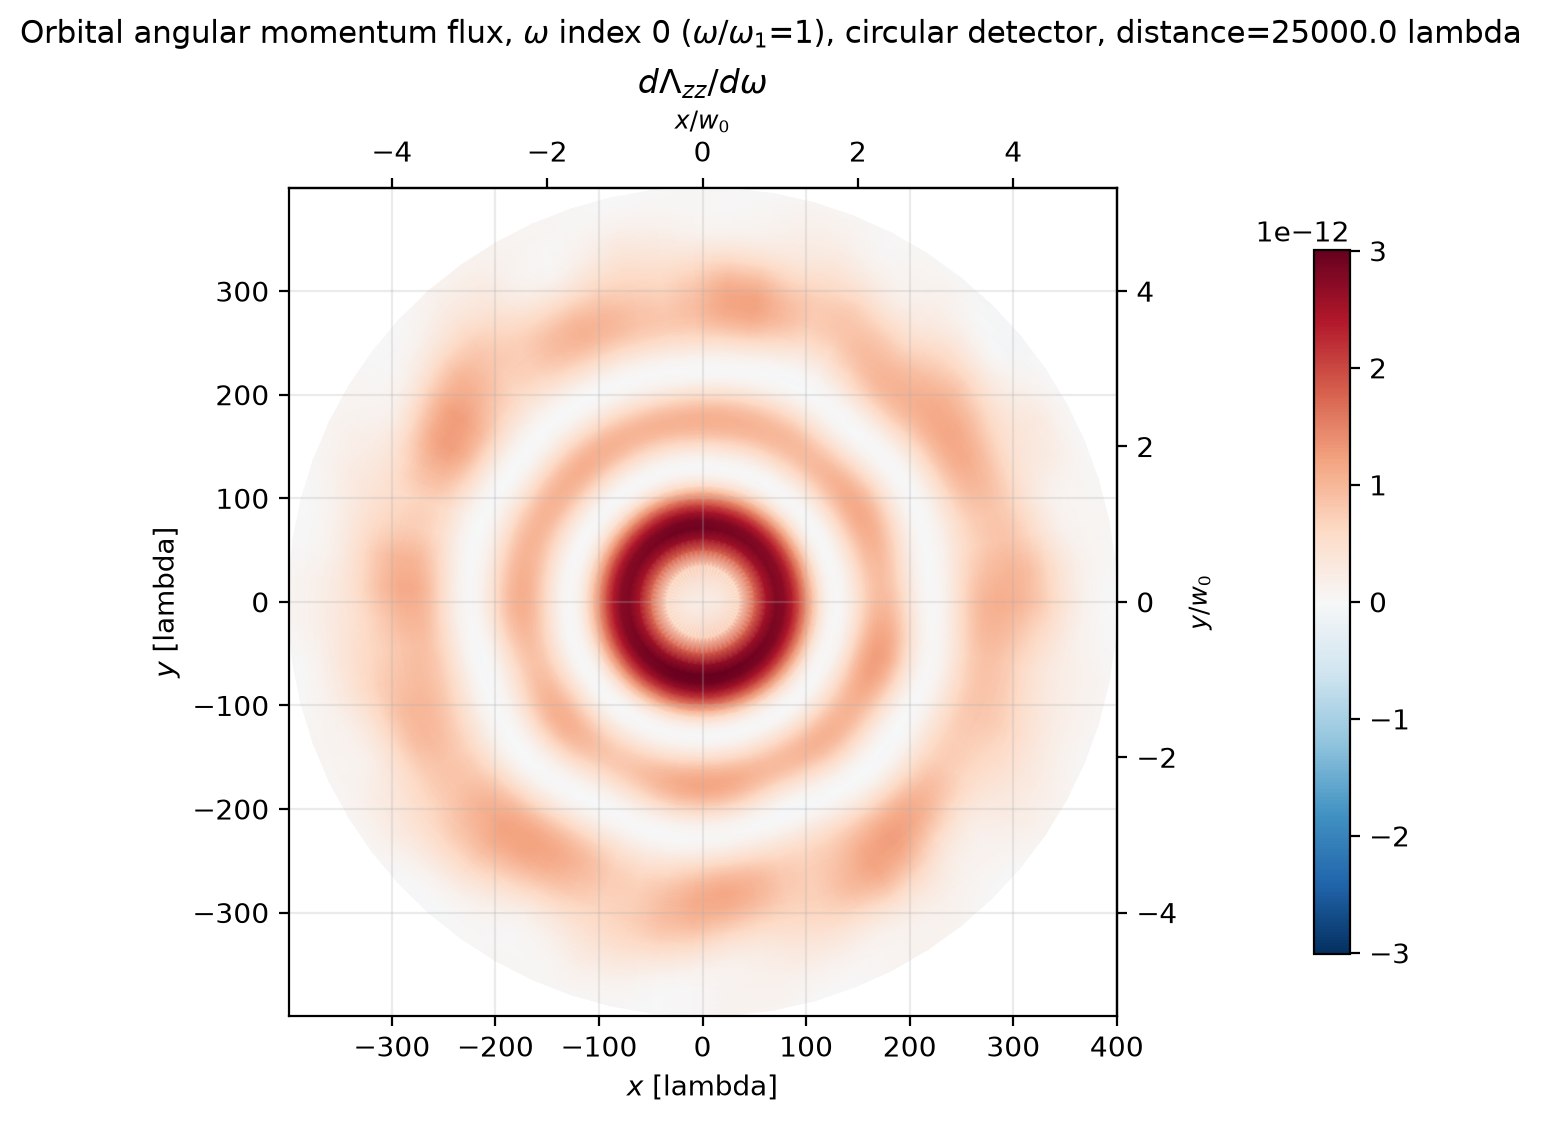
\includegraphics[scale=0.3]{figs/observable_flux_orbital_omega0.png} \hspace{0.5cm}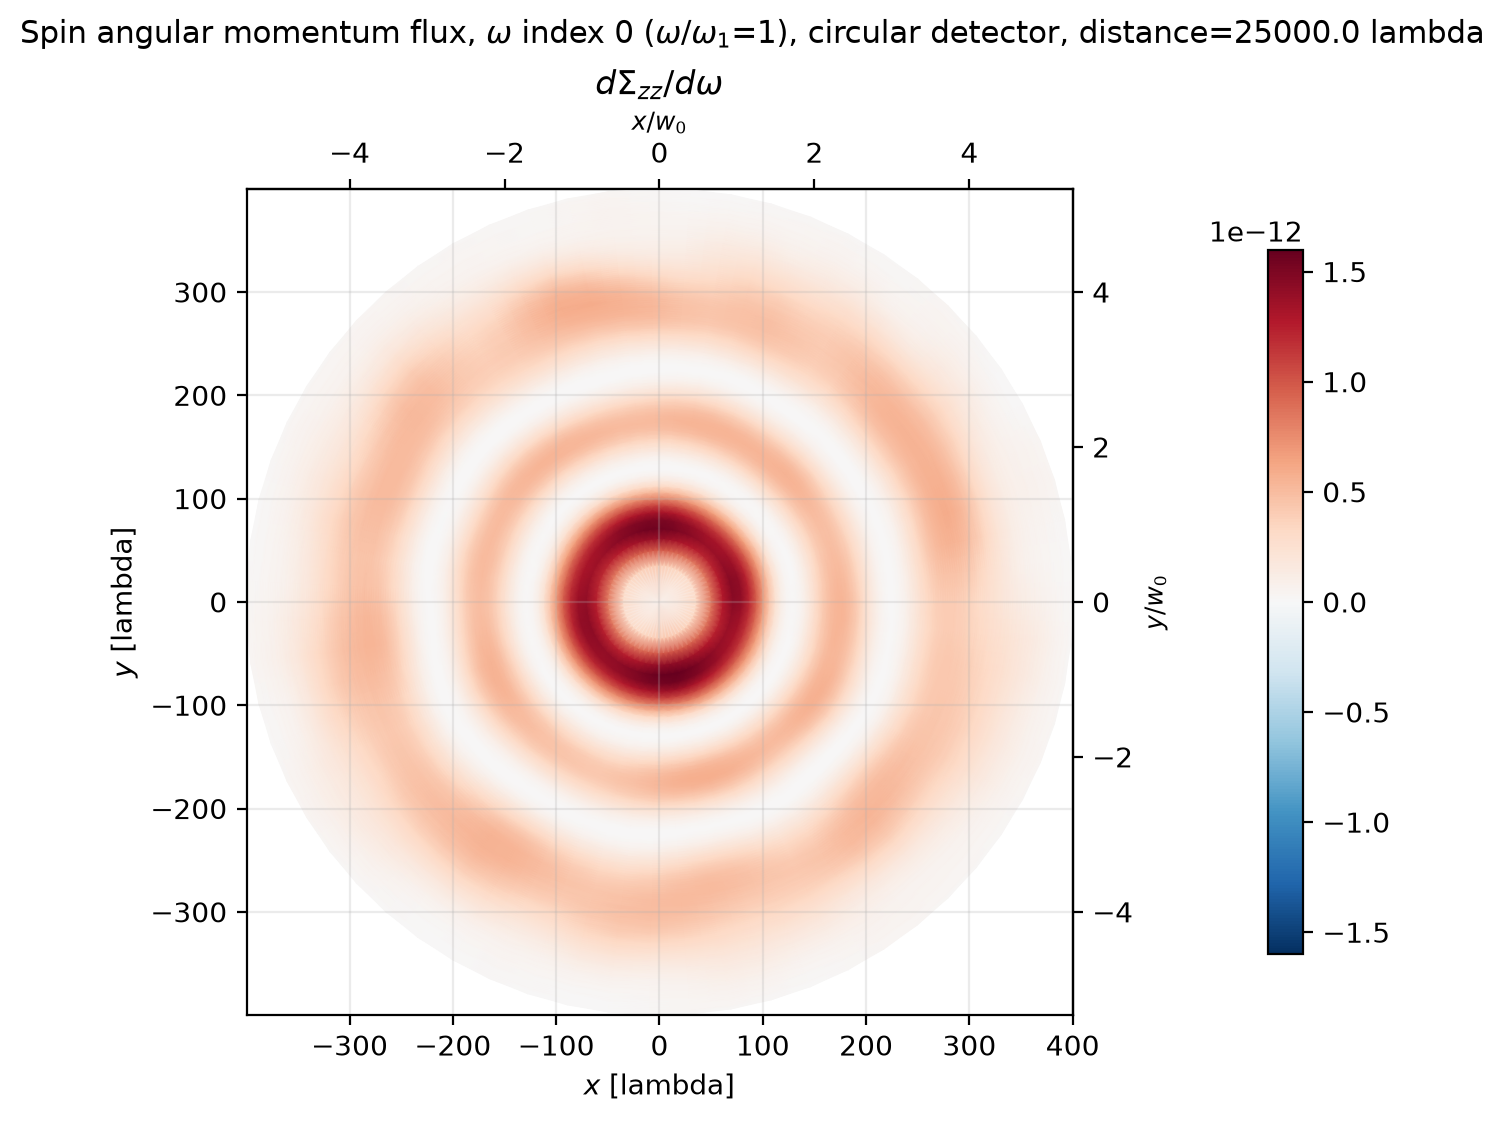
\includegraphics[scale=0.3]{figs/observable_flux_spin_omega0.png}
  \par}

  Orbital and spin flux on the screen for the first harmonic; circularly polarized incident flux, $m=2$
  \begin{columns}[T,onlytextwidth]
    \begin{column}{0.49\textwidth}
      \begin{validationtest}{3}{Orbital-to-spin flux ratio}
        \tiny
        The orbital angular momentum flux is twice the spin flux to high numerical accuracy,
        $d\Lambda_{zz}/d\omega\simeq2\,d\Sigma_{zz}/d\omega$, in agreement with $m=2$.
      \end{validationtest}
    \end{column}
    \begin{column}{0.49\textwidth}
      \begin{validationtest}{4}{Transport at the speed of light}
        \tiny
        Both screen-integrated flux/density ratios agree with $c$ to high numerical accuracy, as for the energy:
        $\frac{\int dS\,d\Lambda_{zz}/d\omega}{\int dS\,d{\cal L}_z/d\omega}
        \simeq\frac{\int dS\,d\Sigma_{zz}/d\omega}{\int dS\,d{\cal S}_z/d\omega}\simeq c$.
      \end{validationtest}
    \end{column}
  \end{columns}
\end{frame}

\begin{frame}{The calculation of the observables of the field}
  \framesubtitle{Numerical example}
  {\par\centering
    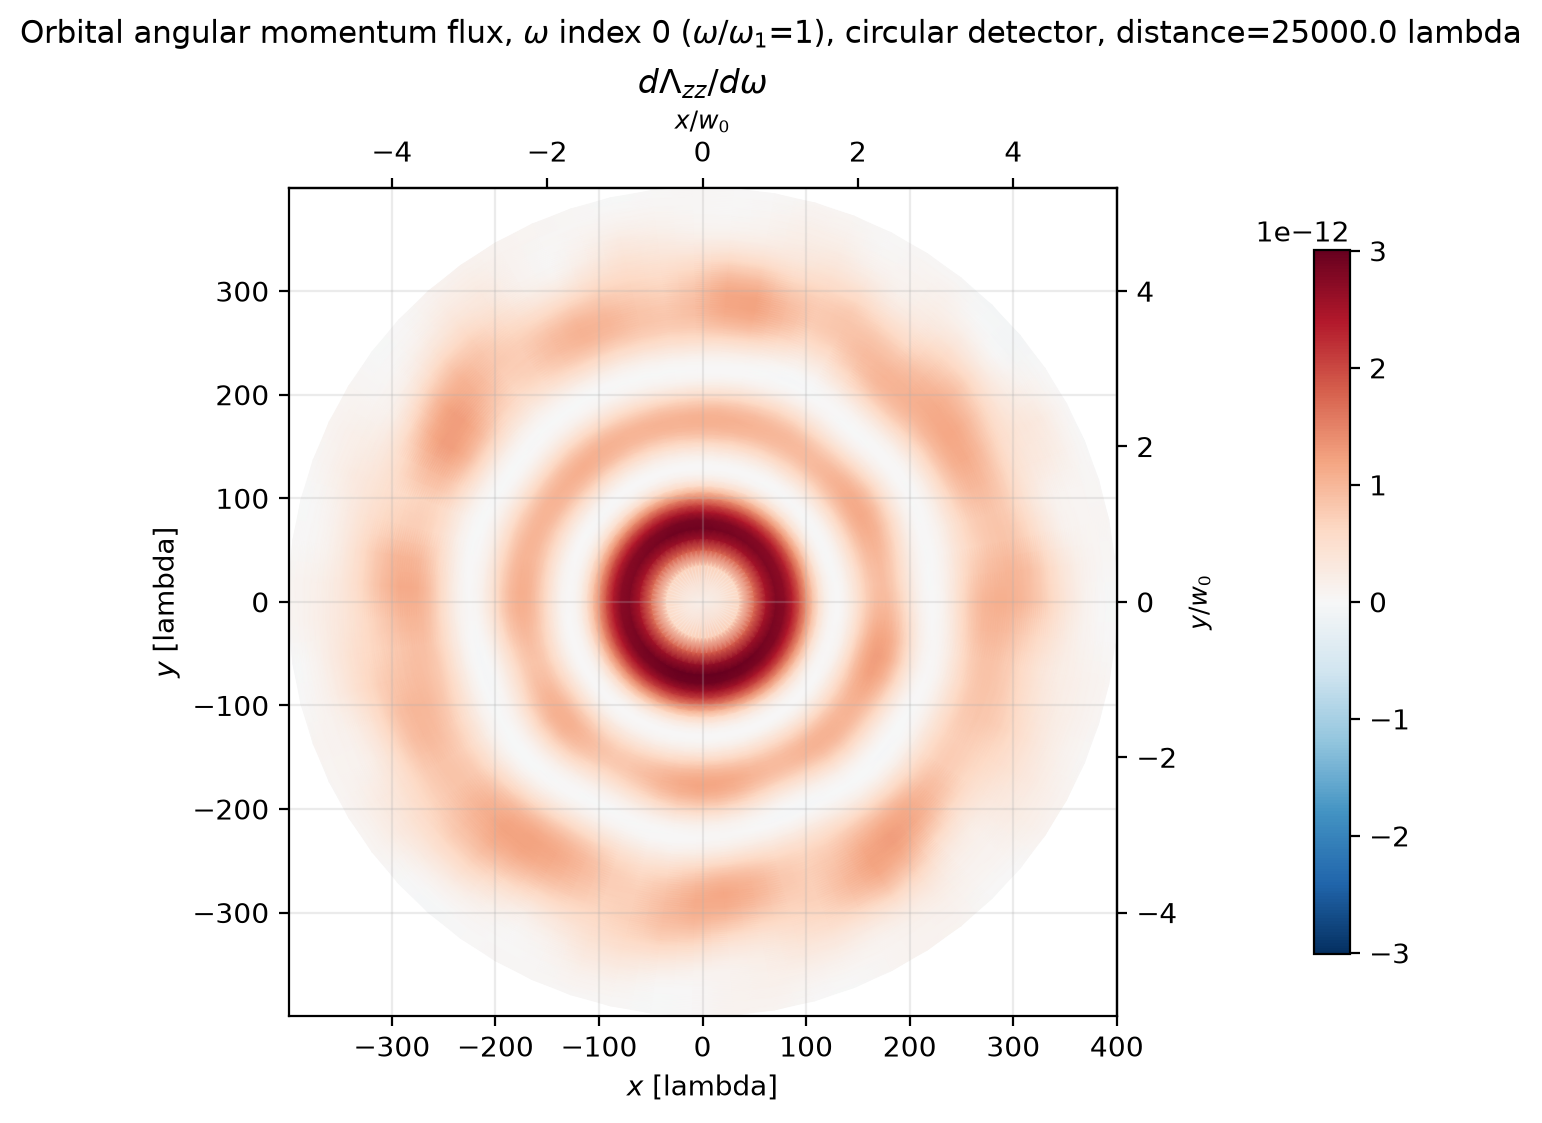
\includegraphics[scale=0.3]{figs/observable_flux_orbital_omega0-lin.png} \hspace{0.5cm}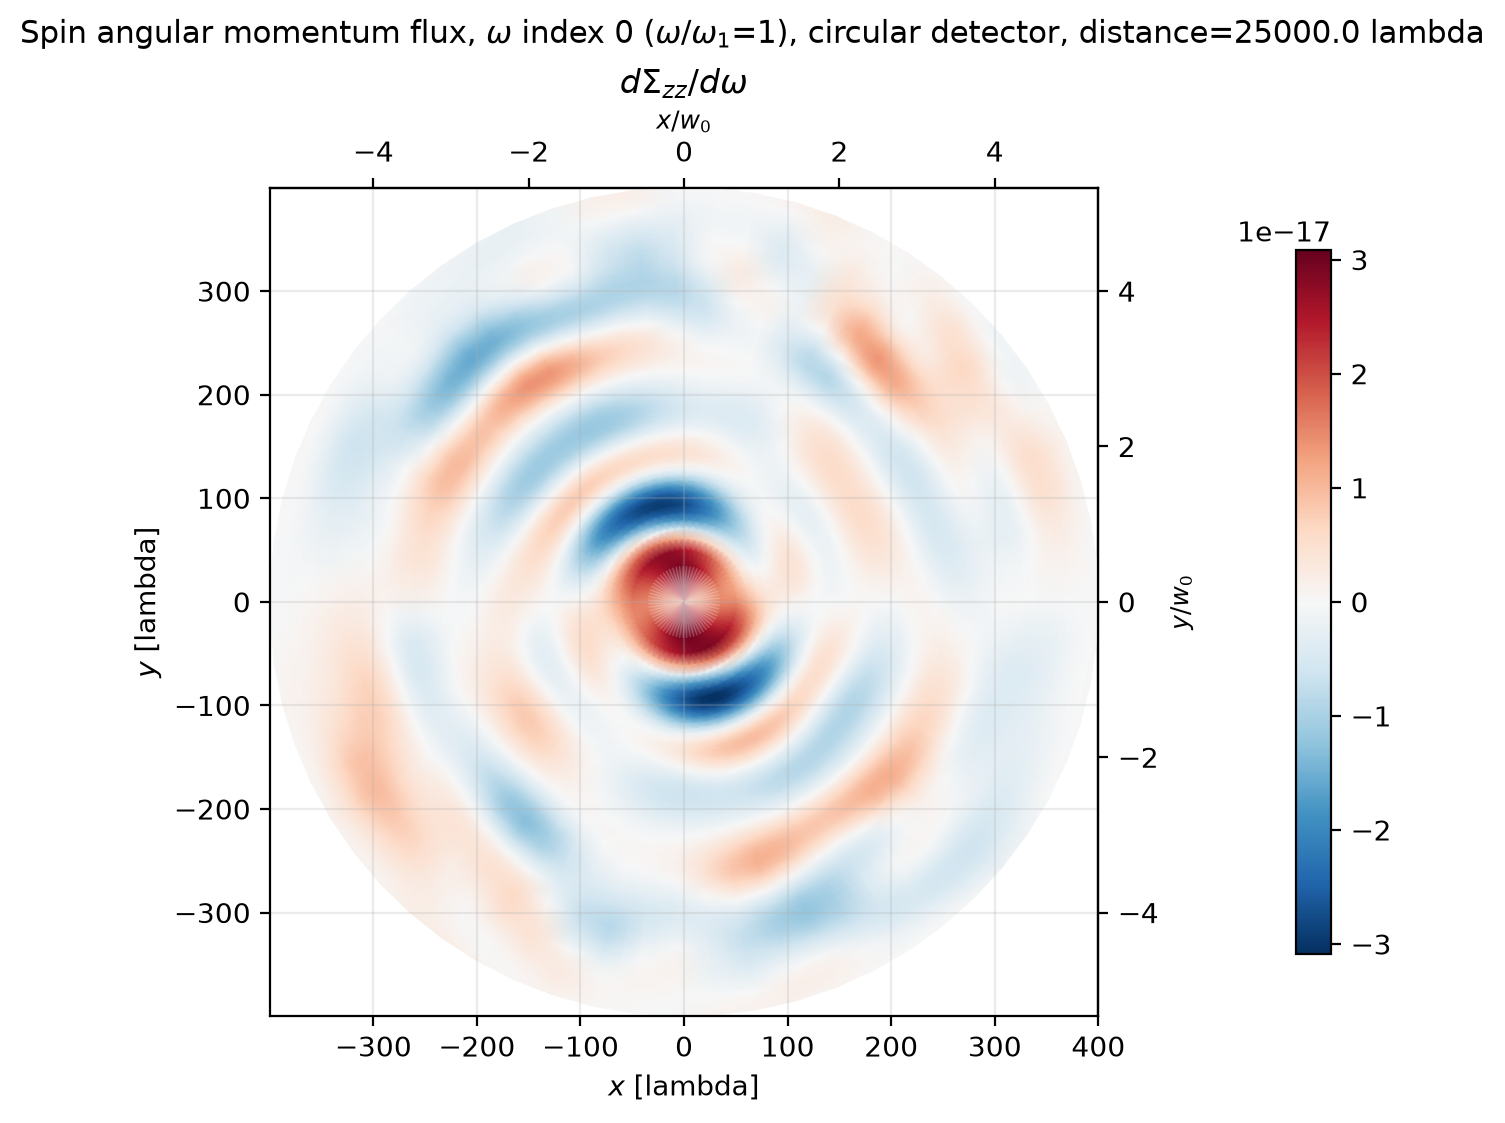
\includegraphics[scale=0.3]{figs/observable_flux_spin_omega0-lin.png}
  \par}

  Orbital and spin flux on the screen for the first harmonic; linearly polarized incident flux, $m=2$
  \begin{columns}[T,onlytextwidth]
    \begin{column}{0.49\textwidth}
      \begin{validationtest}{5}{Vanishing emitted spin}
        \tiny
        For linear incident polarization, the emitted spin angular momentum is zero:
        $d\Sigma_{zz}/d\omega\simeq0$ within numerical accuracy.
      \end{validationtest}
    \end{column}
    \begin{column}{0.49\textwidth}
      \begin{validationtest}{6}{Orbital angular momentum / energy}
        \tiny
        Screen-integrated ratio:
        $\frac{\int dS\,d{\cal L}_z/d\omega}{\int dS\,du/d\omega}=34.524738132$.\\
        Theoretical $m/\omega=35.09$; relative deviation: $1.61\%$.
      \end{validationtest}
    \end{column}
  \end{columns}
\end{frame}

\section{Further validation and new features}
\begin{frame}{Further validation and new features}
  \theorylabel the code computes the emitted field and energy/angular momentum observables,
  with initial validation completed for the fundamental harmonic.
  \par\medskip
  \begin{columns}[T,onlytextwidth]
    \begin{column}{0.48\textwidth}
      \begin{block}{Further validation of the existing code}
        \begin{itemize}
          \item Compare different analytical formulas for the angular momentum and verify their numerical agreement.
          \item Test the OAM/SAM ratio and the ratios of screen-integrated flux to screen-integrated density
            for different laser intensities and for electrons initially in motion.
          \item Study higher harmonics; preliminary results appear satisfactory, but further validation is needed.
          \item Compare the results with Gabriel's equivalent code for the same physical parameters and initial conditions.
        \end{itemize}
      \end{block}
    \end{column}
    \begin{column}{0.48\textwidth}
      \setbeamercolor{block title}{fg=DarkSlate,bg=AmberAlert!15!white}
      \setbeamercolor{block body}{fg=DarkSlate,bg=AmberAlert!4!white}
      \begin{block}{New features to be implemented}
        \begin{itemize}
          \item Implement the long-distance approximation to simplify the analytical formulas and potentially reduce the running time.
          \item Integrate over the full spectral line profile, extending the calculation beyond a single frequency.
          \item Address the screen-distance scaling $d\propto\gamma^2$, where $\gamma$ is the electron Lorentz factor:
            the required distance becomes impractically large, even on macroscopic scales.
        \end{itemize}
      \end{block}
    \end{column}
  \end{columns}
\end{frame}

\end{document}
